\documentclass[11pt,a4paper]{article}
\usepackage[margin=25mm, headheight=14pt]{geometry}
% Shared preamble: fonts, colours, code listings, tables.
\usepackage[T1]{fontenc}
\usepackage[utf8]{inputenc}
\usepackage{lmodern}
\usepackage{microtype}
\usepackage{amsmath}
\usepackage{graphicx}
\usepackage{booktabs}
\usepackage{tabularx}
\usepackage{longtable}
\usepackage{enumitem}
\usepackage{float}
\usepackage[table]{xcolor}
\usepackage{listings}
\usepackage{caption}
\usepackage{titlesec}
\usepackage{fancyhdr}
\usepackage{xurl}
\usepackage[hidelinks]{hyperref}

\graphicspath{{../figures/}{../../participant-kit/figures/}{../../data/}}

% Colours lifted from participant-kit/plotstyle.py, so the document and the
% charts in it are the same palette.
\definecolor{ink}{HTML}{0B0B0B}
\definecolor{inksoft}{HTML}{52514E}
\definecolor{inkmuted}{HTML}{8A8983}
\definecolor{accent}{HTML}{2A78D6}
\definecolor{warn}{HTML}{EC835A}
\definecolor{good}{HTML}{0CA30C}
\definecolor{rule}{HTML}{E6E5E1}
\definecolor{surface}{HTML}{FCFCFB}

\hypersetup{colorlinks=true, linkcolor=accent, urlcolor=accent}

\captionsetup{font=small, labelfont={bf,color=ink},
              textfont={color=inksoft}, skip=6pt}
\captionsetup[table]{skip=4pt}

\titleformat{\section}{\Large\bfseries\color{ink}}{\thesection}{0.7em}{}
\titleformat{\subsection}{\large\bfseries\color{ink}}{\thesubsection}{0.7em}{}
\titleformat{\subsubsection}{\normalsize\bfseries\color{inksoft}}%
            {\thesubsubsection}{0.7em}{}
\titlespacing*{\section}{0pt}{2.2ex plus 1ex minus .2ex}{1.2ex plus .2ex}

\pagestyle{fancy}
\fancyhf{}
\fancyhead[L]{\small\color{inkmuted}TYTFS 2024 as a PyPSA network}
\fancyfoot[C]{\small\color{inkmuted}\thepage}
\renewcommand{\headrulewidth}{0.4pt}
\renewcommand{\footrulewidth}{0pt}

\lstdefinestyle{code}{
  basicstyle=\ttfamily\scriptsize\color{ink},
  keywordstyle=\color{accent}\bfseries,
  commentstyle=\color{inkmuted}\itshape,
  stringstyle=\color{good},
  numberstyle=\ttfamily\tiny\color{inkmuted},
  backgroundcolor=\color{surface},
  frame=leftline, framerule=1.6pt, rulecolor=\color{rule},
  framexleftmargin=6pt, xleftmargin=10pt,
  breaklines=true, breakatwhitespace=true,
  showstringspaces=false, tabsize=4,
  aboveskip=1.1em, belowskip=1.1em,
  columns=fullflexible, keepspaces=true,
}
\lstset{style=code, language=Python}
\lstdefinelanguage{shell}{morekeywords={python,pip,pytest,git},
  sensitive=true, morecomment=[l]{\#}}

% \code{...} for an inline identifier, \file{...} for a path.
\newcommand{\code}[1]{\texttt{\small #1}}
\newcommand{\file}[1]{\texttt{\small\color{inksoft} #1}}
% \where{file}{symbol} - the standard "this lives here" pointer.
% A long identifier list has no break points once it is in \texttt, so the
% box is set ragged-right with plenty of stretch rather than overfull.
\newcommand{\where}[2]{\par\smallskip\noindent%
  \begingroup\small\color{inksoft}\raggedright\emergencystretch=3em%
  \textbf{Code:}~\texttt{#1}~$\rightarrow$~\texttt{#2}\par\endgroup\smallskip}

\setlist[itemize]{leftmargin=1.3em, itemsep=2pt, topsep=4pt}
\setlist[enumerate]{leftmargin=1.6em, itemsep=2pt, topsep=4pt}
\renewcommand{\arraystretch}{1.15}


\title{\vspace{-1.5cm}\bfseries Ireland's electricity network from public data\\[2mm]
\large\mdseries\color{inksoft} What was built, where every number comes from,
and what the result supports}
\author{\normalsize\color{inksoft} Built with Claude Code}
\date{\normalsize\color{inksoft}\today}

\begin{document}
\maketitle
\thispagestyle{empty}

\begin{abstract}
\noindent
This repository builds two things from published data. The first is a
measurement of how much of Ireland's electricity network OpenStreetMap
actually contains, which decides whether volunteer mapping can stand in for
the distribution operator's own records. The second is a working power-system
model: EirGrid's four published planning cases converted into PyPSA networks,
given coordinates from OpenStreetMap, cut down to a study region, fitted with
a week of hourly profiles, and packaged so that somebody else can run them.

This document is the guide to both. Its first job is provenance. Every figure
quoted here traces to a named file, produced by a named function, from a
source that is named with its publisher and its terms. Section~\ref{sec:sources} is that
register, written for a reader who wants to know what is being relied on
before reading what was concluded from it.

Three of the sources could not be reached from the machine this work was done
on. Where that changed what could be delivered, the section says so and says
what is standing in for the missing data.
\end{abstract}

\vspace{4mm}
\noindent\colorbox{surface}{%
\begin{minipage}{\dimexpr\textwidth-2\fboxsep}
\small
\textbf{The short version.}
\begin{itemize}[leftmargin=1.2em]
\item OpenStreetMap carries the Irish network well at 38~kV and above and
      barely at all below it: 22\% of the sub-110~kV line length, 2\% of the
      distribution transformers.
\item Four EirGrid planning cases become eight PyPSA networks. All are
      connected, all solve a DC power flow, all solve a linear optimisation
      with HiGHS.
\item The conversion is checked against each case's own solved voltage angles.
      Correlation is 0.99 or better on seven of the eight networks.
\item 87\% of transmission buses were placed from OpenStreetMap names, and
      those placements sit a median of \textbf{14~metres} from EirGrid's own
      published station coordinates.
\item Two methods that share no data beyond the network itself pick the same
      binding circuit: Letterkenny to Strabane, the 110~kV tie into Northern
      Ireland.
\item Every hour of weather in the shipped networks was generated here. No
      hour of it ever happened, and Section~\ref{sec:hours} says exactly what
      that does and does not permit.
\end{itemize}
\end{minipage}}

\clearpage
\tableofcontents
\clearpage

% ===================================================================
\section{What is in this repository}

Two bodies of work share the checkout. They meet on one question: how much of
Ireland's electricity system can be reconstructed from data anyone can
download?

\textbf{The coverage study} asks whether OpenStreetMap can supply the
distribution network for an energy-system model, and measures the answer
instead of assuming one. It reads a national OpenStreetMap extract and
EirGrid's own asset register, compares them against each other and against
ESB Networks' published totals, and draws the result. Five modules do the
work: \file{network.py}, \file{eirgrid.py}, \file{analysis.py},
\file{plots.py}, and a trio that builds a self-contained interactive map.
Its conclusions are in \file{FINDINGS.md} and summarised in
Section~\ref{sec:osm}.

\textbf{The model build} takes the four PSS/E load-flow cases EirGrid
publishes with its Ten Year Transmission Forecast Statement and turns them
into something a study can run on. \file{psse.py} reads the file format,
\file{pypsa\_net.py} converts it, \file{geocode.py} adds geography,
\file{northwest.py} extracts a region and checks it against a hand-built
dataset, \file{profiles.py} and \file{synthetic.py} supply hours, and
\file{build\_kit.py} assembles a standalone kit.

\file{graph-workshop/} is a separate teaching project that happens to sit in
the same checkout. It shares no code and no data with either half.

\subsection{Running it}

The coverage study rebuilds from a 392~MB download:

\begin{lstlisting}[language=shell]
python network.py prepare        # download, verify, prefilter, cache boundaries
python analysis.py all           # the five measurements -> data/*.json
python eirgrid.py fetch          # EirGrid's own asset register -> GeoPackage
python plots.py all              # every map
\end{lstlisting}

The model build needs no download at all, because the study files and the
OpenStreetMap substation list are both committed:

\begin{lstlisting}[language=shell]
python geocode.py match data/TYTFS2024_studyfiles/*_V35.raw
python pypsa_net.py build        # -> data/pypsa/<case>_<scope>/
python pypsa_net.py verify       # connectivity, DC power flow, optimisation
python northwest.py extract      # the North-West region, both views
python synthetic.py build        # a seeded year of profiles
python build_kit.py              # -> participant-kit/
python -m pytest                 # 215 tests
\end{lstlisting}

The participant kit is a directory that can be lifted out whole. Nothing in it
imports anything from the build half:

\begin{lstlisting}[language=shell]
cd participant-kit
python -m venv .venv && source .venv/bin/activate
pip install -r requirements.txt
python examples/a_dc_power_flow.py
\end{lstlisting}

Measured from a clean virtual environment, that takes 42 seconds and ends in a
plotted map.

Every stage caches into \file{data/raw/} and skips itself when the cache is
present, so the commands are safe to repeat and there is no order to remember.

% ===================================================================
\clearpage
\section{Where the data comes from}
\label{sec:sources}

Ten sources, of which seven are used, one is used only as a set of published
totals to compare against, and two could not be reached.

\begin{table}[H]\centering\small
\begin{tabularx}{\textwidth}{lXl}
\toprule
\textbf{source} & \textbf{what it is and how it arrives} & \textbf{read by} \\
\midrule
\href{https://cms.eirgrid.ie/all-island-ten-year-transmission-forecast-statement-2024}{TYTFS 2024 study files} &
EirGrid and SONI's four published PSS/E v35 load-flow cases for the all-island
system. Committed to \file{data/TYTFS2024\_studyfiles/}, so nothing is fetched
at run time. &
\file{psse.py} \\
\addlinespace
\href{https://services-eu1.arcgis.com/1VGs4Se8lewgdzfE/arcgis/rest/services/TDP_2024_Web_Map_PUBLIC/FeatureServer}{Transmission Development Plan 2024} &
EirGrid's own asset register, published as an anonymous ArcGIS feature
service. Three layers: overhead line, underground cable, stations. Downloaded
page by page and cached as a GeoPackage. &
\file{eirgrid.py} \\
\addlinespace
\href{https://download.geofabrik.de/europe/ireland-and-northern-ireland.html}{OpenStreetMap national extract} &
Geofabrik's island-wide extract, 392~MB, checksum verified, then filtered
down to the 761{,}470 objects carrying a \code{power} tag. &
\file{network.py} \\
\addlinespace
\href{https://www.openstreetmap.org}{OpenStreetMap substations} &
Every named \code{power=substation} and \code{power=plant} on the island, from
the Overpass API. 1{,}705 objects, committed as
\file{data/osm\_substations.csv}. &
\file{geocode.py} \\
\addlinespace
\href{https://services6.arcgis.com/MmUrOQU5v1he9gfS/arcgis/rest/services/Counties_OSi_Ireland/FeatureServer/0}{County boundaries} &
The 26 Republic of Ireland counties, from Ordnance Survey Ireland's statutory
boundary service via Esri Ireland. &
\file{eirgrid.py} \\
\addlinespace
\href{https://www.esbnetworks.ie/about-us/company/our-network}{ESB Networks asset counts} &
Published headline figures for the distribution network. Used only as
denominators, never as geometry. &
\file{analysis.py} \\
\addlinespace
Hand-built node list &
Three spreadsheets supplied with the brief, describing the North-West region
as 24 and then 15 nodes. Committed unchanged to \file{data/handbuilt/}. &
\file{northwest.py} \\
\addlinespace
\href{https://open-meteo.com/en/docs/historical-weather-api}{ERA5 through Open-Meteo} &
Reanalysis weather, which would supply real hourly wind and solar. \textbf{Never fetched}: the host is refused by
this environment's egress policy. &
\file{profiles.py} \\
\addlinespace
EirGrid Smart Grid Dashboard &
Published all-island demand and wind generation, which would supply the demand
shape and validate the wind profiles. \textbf{Never fetched}, same reason. &
\file{profiles.py} \\
\addlinespace
Synthetic profiles &
Generated in this repository from the case files alone, seeded with 42. This
is the only source of hours in the shipped networks. &
\file{synthetic.py} \\
\bottomrule
\end{tabularx}
\caption{The source register. Everything downstream is built from these and
from nothing else.}
\end{table}

\subsection{The TYTFS study files, in plain terms}

EirGrid and SONI operate the transmission systems of the Republic and Northern
Ireland. Once a year they publish a forecast of what that system will look
like a decade out, and with it they release the working files behind it: four
load-flow cases, each a snapshot of the whole island at one moment, solved.

A case is a plain text file listing every busbar, every circuit, every
transformer and every machine, with the electrical properties of each and the
answer the operator's own software produced for it. The four differ in two
ways. Two are set on the 2024 network and two on the planned 2033 network,
which has more of everything. Within each pair, one is a winter peak, when
demand is highest, and one is a summer valley, when it is lowest.

\begin{table}[H]\centering\small
\begin{tabular}{llrrrr}
\toprule
\textbf{case} & \textbf{condition} & \textbf{buses} & \textbf{branches} &
\textbf{machines} & \textbf{running} \\
\midrule
WP2024 & winter peak, 2024 network   & 2{,}025 & 1{,}129 & 597 & 87 \\
SV2024 & summer valley, 2024 network & 1{,}979 & 1{,}120 & 558 & 18 \\
WP2033 & winter peak, 2033 network   & 2{,}457 & 1{,}296 & 847 & 710 \\
SV2033 & summer valley, 2033 network & 2{,}457 & 1{,}296 & 847 & 45 \\
\bottomrule
\end{tabular}
\caption{The four cases as the parser reads them. ``Machines'' is the
generator register, which lists everything connected; ``running'' is how many
of them the case actually dispatches. The gap between those two columns is the
single easiest way to get a wrong answer out of these files, and
Section~\ref{sec:psse} is about it.}
\end{table}

Two things about the files are worth knowing before any number is quoted from
them. They describe a forecast of how the system is planned to develop, and
EirGrid publishes them for reference without warranty. And a case
is one hour, so anything that asks when the network is constrained needs hours
that the files do not contain.

\subsection{EirGrid's own asset register}

The Transmission Development Plan web map is EirGrid publishing where its
circuits and stations are. It is served as an ArcGIS feature service that
anyone can query, in Irish Transverse Mercator, and \file{eirgrid.py} pages
through three of its layers: existing overhead line, existing underground
cable, existing stations.

One check that this really is the register: summing the
geometry gives 5{,}348~km of overhead line and 774~km of cable, 6{,}122~km
together, against EirGrid's published figure of about 6{,}500~km.

\textbf{One documented hole, which the aggregate hides.} The 400~kV layer
contains a single circuit, Moneypoint to Oldstreet, 103~km, which is the
western leg. The 400~kV network continues east from Oldstreet to Dunstown and
on to Woodland, and no circuit for those legs appears in the service at any
voltage. The 110~kV and 220~kV layers can be taken as the register. The 400~kV
layer cannot be taken as the whole 400~kV backbone. \code{eirgrid.py summary}
prints that warning, and Section~\ref{sec:geocode} repeats it where the same
service is used as a validator.

\subsection{OpenStreetMap, entered two different ways}

OpenStreetMap is a map anyone can edit, so it records what volunteers have
traced. That makes it a claim about mapping effort as much as a claim about
the network, which is the whole subject of Section~\ref{sec:osm}. This
repository uses it twice, for two different purposes, through two different
doors.

\textbf{The bulk extract} is a single 392~MB file covering the island,
republished continuously by Geofabrik. \file{network.py} downloads it, checks
it against Geofabrik's published MD5, and streams it through a filter that
keeps only objects carrying a \code{power} tag. The result is about 7~MB and
holds 761{,}470 objects. Overpass was avoided here deliberately: one national
file gives complete coverage in one pass, with no query timeouts, no rate
limits and no result caps, and it makes the whole coverage study reproducible
from one download.

Two practical notes for anyone repeating it. The download had to go over plain
HTTP, because this session's egress policy blocks HTTPS to Geofabrik and to
every OpenStreetMap mirror tried, while allowing port 80; the checksum matched,
which gives integrity checking without authentication. And the prefiltering
pass is there for memory and does not change the selection: the reader used
downstream holds the whole node index in RAM and was killed on the full file
with 15~GB available.

\textbf{The substation query} is small and specific. \file{geocode.py} asks
Overpass for every named \code{power=substation} and \code{power=plant} on the
island, which returns 1{,}705 objects: 1{,}288 substations and 417 plants.
1{,}270 of them carry a voltage tag and 367 are tagged at 110~kV or above.
That list is committed to \file{data/osm\_substations.csv}, so the bus
matching in Section~\ref{sec:geocode} reproduces without a network round trip.

OpenStreetMap data is under the Open Database Licence.

\subsection{ESB Networks' published totals}

ESB Networks is the distribution system operator for the Republic. Its own
\href{https://www.esbnetworks.ie/about-us/company/our-network}{website publishes headline asset counts}: 150{,}000~km of overhead line,
22{,}000~km of underground cable, 2.1 million poles, 242{,}000 pole-mounted
transformers, 21{,}680 ground-mounted substations and 571 primary stations. None of that is geometry and none of it is used as
geometry. It is used once, as the denominator that turns ``OpenStreetMap
contains 37{,}125~km of sub-110~kV line'' into ``OpenStreetMap contains about a
fifth of it''.

The distribution network itself was not available for this work. Getting it
means ESB's CAD files and capacity heatmap, and Section~\ref{sec:osm} ends with
an acceptance test to apply to them when they arrive.

\subsection{The hand-built North-West dataset}

Three spreadsheets came with the brief, describing the North-West of the
country as a small node-and-edge model:

\begin{table}[H]\centering\small
\begin{tabularx}{\textwidth}{lX}
\toprule
\file{nodes.xlsx} & the node list, in two blocks: 24 nodes with generation
sites as nodes of their own, then a substation-only view of 15 \\
\file{transmission.xlsx} & 14 of the 15 stations, with the code, rating and
length columns empty. A template with nothing filled in \\
\file{nodes\_24hr.xlsx} & a half-hourly day for the 15 nodes. Its own README
says it was fabricated, with NumPy seed 42 \\
\bottomrule
\end{tabularx}
\end{table}

They are committed unchanged, because Section~\ref{sec:northwest} is a
line-by-line comparison against them and the reader has to be able to check it.

\subsection{The two sources that could not be reached}
\label{sec:blocked}

\file{profiles.py} is a complete pipeline from reanalysis weather to a capacity
factor per generator, with a validation step against EirGrid's published wind
output. It has never run. Both hosts are refused by this environment's egress
policy at the CONNECT, before any request is made:

\begin{lstlisting}[language=shell]
archive-api.open-meteo.com:443    gateway answered 403 to CONNECT
www.smartgriddashboard.com:443    gateway answered 403 to CONNECT
cms.eirgrid.ie:443                gateway answered 403 to CONNECT
\end{lstlisting}

A 403 at CONNECT is an organisation policy denial. It was not retried and no
mirror was sought, because routing around an egress policy is not this
project's call to make.

The consequence is stated plainly wherever it matters. There are no reanalysis
profiles in this repository and no validation result. What stands in their
place is described in Section~\ref{sec:hours}, and it is generated data with a
seed on it.

\subsection{What is measured, what is inferred, and what was invented}

The distinction runs through everything below, so it is worth one table.

\begin{table}[H]\centering\small
\begin{tabularx}{\textwidth}{lX}
\toprule
\textbf{measured} & Every electrical property of the network: buses, circuits,
impedances, ratings, transformers, the machine register, which buses carry
load and how much. All read out of the TYTFS files. Station coordinates, read
out of OpenStreetMap. Circuit and cable geometry, read out of EirGrid's
register. Mapping coverage, measured off the OpenStreetMap extract. \\
\addlinespace
\textbf{inferred} & What the twelve PSS/E rating columns mean
(Section~\ref{sec:rate}). Which technology each machine is, taken from bus-name
prefixes, which leaves about a fifth labelled \code{unknown}. Which station a
sub-110~kV bus belongs to, taken from least-reactance distance. Ratings for
zero-impedance couplers, taken from what is attached to them. \\
\addlinespace
\textbf{invented} & Every hour of weather. The shape of demand through the day.
Marginal costs. The value put on unserved energy. These are stated wherever
they are used and they are all in the exported CSVs, so a study can replace
them. \\
\bottomrule
\end{tabularx}
\end{table}

\subsection{How the pieces connect}

\begin{lstlisting}[language=shell]
Geofabrik extract ---> network.py ---> analysis.py ---> FINDINGS.md
                              |                \--> plots.py --> maps
                              \--> extract_web_*.py --> build_web_map.py
EirGrid ArcGIS  ------> eirgrid.py ------^  and the geocoding cross-check

TYTFS .raw ----> psse.py ----> pypsa_net.py ----> data/pypsa/<case>_<scope>/
Overpass ------> geocode.py ------^   |
                                      +-------> northwest.py --> the region
                                      +-------> synthetic.py --> the hours
                                                        |
                                              build_kit.py --> participant-kit/
\end{lstlisting}

% ===================================================================
\clearpage
\section{Part I. How much of the network does OpenStreetMap have?}
\label{sec:osm}

The question came from an energy-system model that needed a distribution
network and hoped to avoid asking the utility for one. The answer separates
sharply by voltage, and the separation is the finding.

\begin{figure}[H]\centering
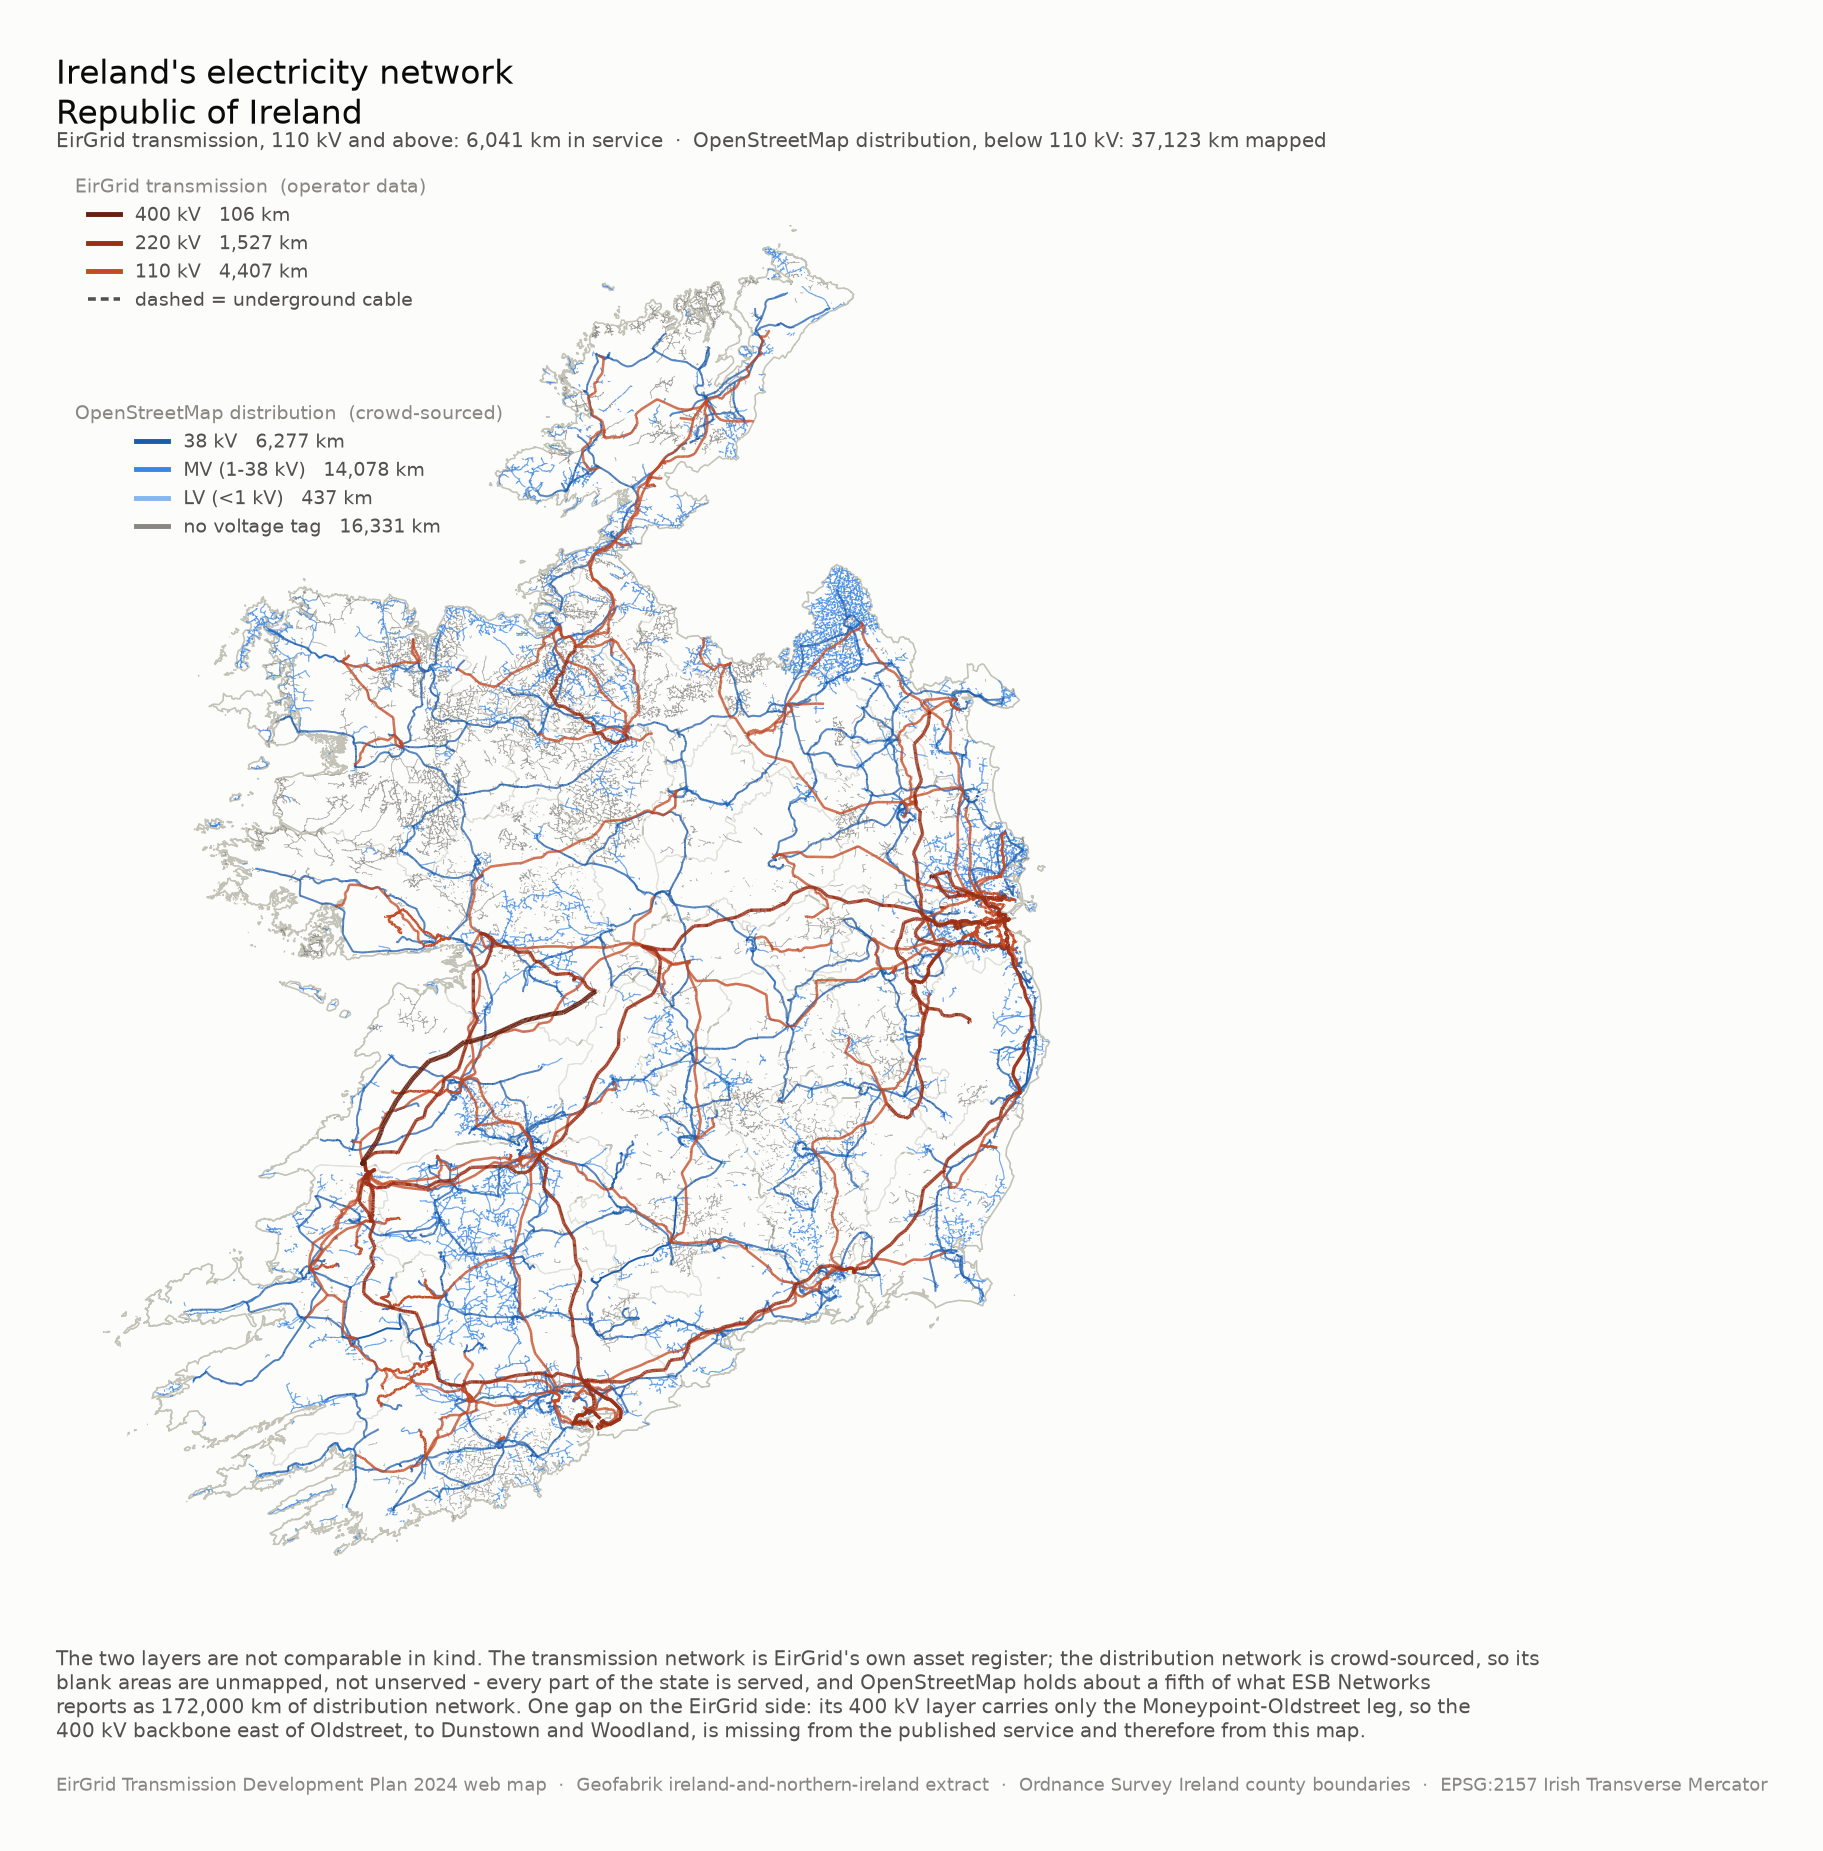
\includegraphics[width=\textwidth]{national_network.png}
\caption{Both layers together. The warm lines are EirGrid's own register at
110~kV and above. The blue lines are what volunteers have traced below that.
The colour families are deliberately far apart, because the two carry different
kinds of claim: blank areas in the blue layer are unmapped rather than
unserved.}
\end{figure}

\subsection{One bug worth reporting on its own}

The brief predicted that a line of the form \code{if gdf.get("voltage"):} would
fail quietly. It does worse than that. When the column is absent the expression
is \code{None} and the branch silently does nothing; when the column is present
it raises, because the truth value of a pandas Series is ambiguous. It never
behaves as intended.

That matters here because the reader used promotes only a fixed set of tags to
columns and leaves the rest in a JSON blob, and \code{voltage} is in the blob.
A default read of County Kilkenny returns 16{,}078 line features with no
voltage column, the branch skips, and the pipeline reports 0\% voltage
coverage. The true figure for Kilkenny is 48.4\%. Nothing crashes, and the
wrong answer confirms the hypothesis the study set out to test.

\where{network.py}{load\_lines(), tag\_series(); test\_network.py pins both cases}

\subsection{Coverage, against the operator's own totals}

Every OpenStreetMap power feature was attributed to a county and the 26
counties of the Republic summed. The attributed area comes to 70{,}296~km$^2$,
within 0.03\% of the state's actual area, which is a reasonable check that the
attribution works.

\begin{table}[H]\centering\small
\begin{tabular}{lrrr}
\toprule
& \textbf{OpenStreetMap} & \textbf{ESB Networks} & \textbf{share} \\
\midrule
Sub-110 kV line        & 37{,}125 km & 172{,}000 km & \textbf{21.6\%} \\
Wooden poles           & 470{,}731   & 2{,}100{,}000 & \textbf{22.4\%} \\
Underground cable      & 927 km      & 22{,}000 km  & 4.2\% \\
MV/LV transformers     & 4{,}982     & 242{,}000    & \textbf{2.1\%} \\
Ground substations     & 987         & 21{,}680     & 4.6\% \\
\bottomrule
\end{tabular}
\caption{The structure of this table is the finding. Line length and pole count
agree at about 22\%, which is two independent measures of the same thing and
suggests roughly a fifth of the rural overhead network has been traced. Cable,
transformers and substations sit at 2 to 5\%, a factor of five worse.
OpenStreetMap has a fifth of the wires and a fiftieth of the plant.}
\end{table}

The transformer figure is the damaging one. Distribution substations are where
a network-derived model would place its buses, and 2\% of them are present.

\textbf{A check that needs no external reference.} Every transformer and
substation OpenStreetMap maps has to be reached by conductor, whatever the real
network looks like. A minimum spanning tree over the mapped assets is therefore
a hard and very generous lower bound on the length required. Dublin City fails
that bound against its own data: 874 mapped transformers and substations,
154~km of tree required, and 7.8~km of sub-38~kV line actually mapped. At least
95\% of Dublin's medium-voltage network is missing, and that follows without
reference to ESB at all.

\where{analysis.py}{counties(), missing\_cable()}

\subsection{Topology: a scattering of segments below 38 kV}

Run island-wide with no county clipping, because clipping cuts every line that
crosses a boundary and would inflate the counts for exactly the layers that
span counties:

\begin{table}[H]\centering\small
\begin{tabular}{lrrrrr}
\toprule
\textbf{layer} & \textbf{km} & \textbf{nodes} & \textbf{components} &
\textbf{largest} & \textbf{share} \\
\midrule
220 kV and above & 2{,}640  & 10{,}241  & \textbf{22}     & 9{,}680  & \textbf{94.5\%} \\
110 kV           & 6{,}190  & 42{,}830  & 124             & 20{,}598 & 48.1\% \\
38 kV            & 6{,}278  & 50{,}416  & 347             & 9{,}608  & 19.1\% \\
38 kV and above  & 15{,}108 & 103{,}301 & 419             & 66{,}047 & 63.9\% \\
MV, 1 to 38 kV   & 23{,}886 & 293{,}381 & \textbf{6{,}707} & 25{,}420 & \textbf{8.7\%} \\
LV, below 1 kV   & 619      & 17{,}495  & \textbf{4{,}682} & 149      & \textbf{0.9\%} \\
\bottomrule
\end{tabular}
\caption{From \file{data/national.json}. The upper layers behave like mapped
infrastructure. The lower ones do not.}
\end{table}

For context on the 6{,}707 medium-voltage components: ESB operates 571 primary
stations nationally, and a radial network has roughly one component per primary
busbar, so the true figure is of order 500 to 600. OpenStreetMap gives an order
of magnitude more. Below 38~kV this is a collection of independently traced
segments rather than a network. Someone walked a run of poles along one road,
someone else walked another two townlands away, and the span between them was
never traced.

\textbf{Snapping does not fix it.} If the fragmentation were imprecise noding,
component count would collapse once the tolerance passed the noding error.
Widening from 0.1~m to 25~m in Kilkenny, already far beyond any plausible
tracing error, removes 18\% of components. At 100~m the graph is being
destroyed faster than it is being joined: node count falls by 68\% while
component count falls by 47\%, and the largest component shrinks from 3{,}777
nodes to 1{,}361 as spurious merges rewire it. The missing spans are hundreds
of metres of unmapped conductor, so no tolerance recovers them.

\where{analysis.py}{national(), analyse\_area(); network.py $\rightarrow$ to\_graph()}

\subsection{Is it worth anything as a spatial prior?}

For the line layer, no. Mapped sub-110~kV density across the 26 counties runs
from 210~km per 1{,}000~km$^2$ in Westmeath to 1{,}450 in Monaghan, a factor of
6.9. The tempting reading is urban against rural, and it does not survive
contact with the list: Monaghan and Westmeath are both small inland counties of
similar character and differ by seven times, while County Dublin, which has the
highest demand density in the state, sits third. What the ranking reproduces is
where an active local mapper happened to work. Using mapped circuit length as a
demand prior would import a sevenfold arbitrary regional distortion, which is
worse than using no spatial information at all because it looks like data.

For the point layer the answer is more useful and comes with a caveat. Dublin
City has 874 mapped transformers and substations in 119~km$^2$ against
Kilkenny's 128 in 2{,}071~km$^2$, a density ratio of about 118 to 1 in the
direction demand actually runs. Those urban substations get mapped because they
are visible street furniture. The caveat is that this density partly measures
mapper effort, mapper effort correlates with urbanity, and urbanity correlates
with demand, so the point layer will look like a good demand prior whether or
not it is one, and OpenStreetMap alone cannot separate the two.

\subsection{The verdict, and what to do with it}

Take the 38~kV-and-above layer. It is 15{,}108~km island-wide, 64\% of its
nodes sit in one component, and above 220~kV that rises to 94.5\%. For placing
regional nodes and constraining transfer between them it is adequate and it is
free.

Do not use anything below 38~kV, as topology or as a demand prior. Go to ESB
for that, and apply two cheap acceptance tests when the data arrives: does the
medium-voltage layer resolve to something near 571 connected components
nationally, and does its conductor length reach the transformer population?
Both are the questions OpenStreetMap fails.

\subsection{The interactive map}

\file{data/ireland\_distribution\_map.html} is the same data as a map that
opens from disk with no server. Three scripts build it: one reassembles the
conductor runs and reduces polygon substations to points, one extracts the
county and Northern Ireland outlines so the map still reads as Ireland with no
tile server, and one inlines every byte of geometry, styling and script into a
single file.

Two decisions carry the file size. Geometry is simplified in Irish Transverse
Mercator at a tolerance chosen per layer, tight for the transmission layers a
reader will zoom into and looser for the untagged fragments they will not, then
delta encoded against a grid about a metre across. Attributes are stored as
arrays against one shared string pool, so ``ESB Networks'' is written once
rather than eleven thousand times. Together those take the payload from roughly
90~MB of GeoJSON to 11~MB.

The default view is the layers that survived scrutiny, which is 38~kV and above
plus the substations. Medium voltage, low voltage and the untagged remainder
are one click away, with the reason stated beside them.

\where{extract\_web\_data.py, extract\_web\_base.py, build\_web\_map.py}{}

% ===================================================================
\clearpage
\section{Part II. Reading the PSS/E cases}
\label{sec:psse}

\file{psse.py} reads the four study files into pandas DataFrames and does
nothing else. No per-unit conversion, no topology, no network object.
Everything downstream of the file is another module's job.

\textbf{Why not a library.} PyPSA has no PSS/E importer, and the
general-purpose readers that exist carry a solver or a whole network model
behind them. The format is eight sections of comma-separated records with one
genuinely awkward record type, so a dependency would cost more than it saves.
The sections this repository does not need are skipped by name, so that
each skip is a decision recorded in the code and not an accident of the file's
order, and an unrecognised section name raises.

\subsection{The format, as verified against the four files}

Encoding is latin-1 and line endings are CRLF. A line beginning \code{0 /}
delimits sections, and its comment names the section that follows it. Each
section opens with one or more \code{@!} comment lines carrying the column
headers. Records are comma-separated, character fields are single or double
quoted, and anything after an unquoted \code{/} is a comment. Trailing fields
may be omitted, so a short record is padded; a record longer than its layout
raises, because that means the layout is wrong.

Two record types span several lines and are assembled into one flat row so that
every section comes back as a rectangle. A transformer is four lines when it is
two-winding and five when three-winding, and the third field on the first line
says which. A two-terminal DC link is always three lines: link, rectifier,
inverter.

The transformer assembly is checked with arithmetic. WP2024's
transformer section holds 5{,}349 data lines, and the reader finds 1{,}201
two-winding and 109 three-winding records. $1201 \times 4 + 109 \times 5 =
5349$ exactly, with nothing left over. That is the failure mode that matters:
one mis-sized record slides every record after it by a line, and the result
still parses.

\subsection{Validation, and the four checks that did not agree}

Sixteen figures for WP2024 were supplied for the parser to reproduce. Twelve
match exactly, including every voltage count, the branch classification, the
in-service machine count and the dispatched megawatts. Four do not, and both
causes were traced.

Three of them are record counts, each high by exactly one: buses, branches and
loads. Each of those sections carries exactly one \code{@!} header line, and
counting the lines between the two delimiters, instead of the records inside
them gives the three expected figures precisely. The generator count is the
tell: it agreed at 597, and the generator section has a header too, so a
header-inclusive count there would have given 598.

The fourth is the load total, and it is the more interesting one. The expected
8{,}246~MW reproduces exactly as the sum over all 266 load records. What
differs is which records to count. Thirty-four of them are switched out, they
total 921.9~MW, every one carries the same identifier \code{MI}, and every one
sits at a bus that already carries an in-service load record. They are an
alternative representation of the same demand, deliberately disabled. The
solved case settles it: in-service generation is 7{,}411.6~MW against
in-service load of 7{,}324.5~MW, a gap of 1.2\% that is the right size for
losses, while against the full register generation would fall 835~MW short, and
a solved load flow does not fail to serve 10\% of its demand.

\subsection{The in-service flag, and why it is the first thing to check}

WP2024's generator section is a register of 597 machines totalling 18{,}158~MW,
more than twice the island's winter peak. Filtering to in-service leaves 87
machines and 7{,}412~MW, which is a plausible winter-peak dispatch. The
in-service fraction is not stable enough to approximate:

\begin{table}[H]\centering\small
\begin{tabular}{lrrr}
\toprule
& \textbf{records} & \textbf{in service} & \textbf{fraction} \\
\midrule
WP2024 & 597 & 87  & 15\% \\
SV2024 & 558 & 18  & 3\% \\
WP2033 & 847 & 710 & 84\% \\
SV2033 & 847 & 45  & 5\% \\
\bottomrule
\end{tabular}
\end{table}

The reader itself does not filter, because a reader reads. Its
\code{generators()} and \code{loads()} helpers filter by default, and
\code{summary()} reports the in-service and register totals side by side so
neither is hidden.

\where{psse.py}{read\_raw(), read\_all(), generators(), loads(), ac\_branches(), summary()}

\subsection{Three notes for what comes next}

\textbf{Branch counts are unfiltered by default.} 679 AC circuits in WP2024
have both ends at 110~kV or above, of which 645 are in service. Both figures
are defensible, and a downstream model should say which it used.

\textbf{AC circuits never change voltage.} All 679 join two buses at the same
base kV, so classifying a circuit by voltage is unambiguous. Transformation
lives entirely in the transformer section, and a test pins that.

\textbf{The interconnectors are not all in one place.} The two-terminal DC
section holds only Moyle. East-West and Greenlink are modelled as buses with
generator records instead. Anything that needs the island's cross-border
exchange has to look in both places.

% ===================================================================
\clearpage
\section{Part III. Turning a case into a PyPSA network}
\label{sec:conversion}

Six decisions matter, in the specific sense that getting one wrong produces a
network that still solves and whose every downstream number is wrong. Each is
below with the measurement behind it.

\subsection{The per-unit base: 100 MVA, read out of the header}

Every case opens with \code{SBASE = 100.00} and \code{BASFRQ = 50}. The build
asserts it and refuses a case on any other base, because a case on 200~MVA
would produce a network that solves and whose every impedance is out by exactly
two.

PSS/E gives impedances per-unit on that base and on the bus's kV. PyPSA wants
ohms for a line and per-unit on its own rating for a transformer, so there are
two conversions:

\begin{table}[H]\centering\small
\begin{tabular}{lll}
\toprule
& \textbf{PyPSA units} & \textbf{conversion} \\
\midrule
\code{Line.r}, \code{Line.x}    & ohms & $R_{pu}\times \mathrm{kV}^2/100$ \\
\code{Line.b}                   & siemens & $B_{pu}\times 100/\mathrm{kV}^2$ \\
\code{Transformer.r}, \code{.x} & pu on its own \code{s\_nom} & $X_{pu}\times \mathrm{s\_nom}/100$ \\
\bottomrule
\end{tabular}
\end{table}

Transformer records carry their own convention flags and all four cases use the
same ones, with two exceptions on a different impedance base that are rebased
explicitly. A third convention, load loss in watts, does not occur, and
encountering it raises.

\where{pypsa\_net.py}{\_ohms(), \_siemens(), \_z\_on\_system\_base()}

\subsection{RATE1 is taken as the rating, by inference from the data}
\label{sec:rate}

PSS/E v35 carries up to twelve rating slots per branch. RATE1, RATE2 and RATE3
are populated here and RATE4 to RATE12 are zero everywhere.

\textbf{A caveat this report owes the reader.} Siemens' own manual, which would
say what the format fixes about their meaning, is not publicly available.
\href{https://powsybl.readthedocs.io/projects/powsybl-core/en/latest/grid_exchange_formats/psse/}{Open-source readers} document the older three-rating layout without settling
the semantics of the twelve-rating one. What follows is an inference from the
data.

Two facts, measured across all four cases and re-derived for this draft:

\begin{itemize}
\item \code{RATE1 == RATE2} in \textbf{every one of the 4{,}841 branch records}
      across the four cases: 1{,}129 in WP2024, 1{,}120 in SV2024 and 1{,}296
      in each 2033 case. Exactly, not approximately.
\item \code{RATE3/RATE1} is 1.0 or 1.1 in the two winter cases. The two summer
      cases add a third value, 1.10021, on 97 records, which is a rating that
      was rounded before it was written.
\end{itemize}

The natural reading is the normal, long-term-emergency and
short-term-emergency convention, with the long-term rating set equal to the
normal one and the short-term rating at 110\%. The magnitudes agree: the median
RATE1 by voltage in WP2024 implies 659~A at 110~kV and 1{,}475~A at 220~kV,
which are continuous circuit ratings.

\code{s\_nom} therefore takes RATE1, the most conservative of the three. If
that reading is wrong, the direction of the error is known: \code{s\_nom} would
be too small and every loading figure here too high. All three columns are
exported, so a contingency study can pick a different one.

\where{pypsa\_net.py}{CONTINUOUS\_RATE; test\_pypsa\_net.py $\rightarrow$ test\_rate2\_equals\_rate1}

\subsection{The 18 unrated branches, and what they turned out to be}

Eighteen AC branches at 110~kV and above carry no rating in WP2024: nine at
\code{RATE1 = 9999} and nine at \code{RATE1 = 0}. Zero is the more dangerous of
the two because it looks like a number, and putting it into \code{s\_nom} makes
the element unusable and the optimisation infeasible.

Looking at what they are settles the treatment. All eighteen have $R = 0$,
$|X| \leq 0.01$, $B = 0$ and zero length, as do all twenty in each 2033 case.
Every one is a station coupler: a busbar section, a capacitor or reactor stub,
an SVC, a generator terminal tie. None is a circuit whose rating was forgotten,
and a test pins that, because if it stops being true the rule below is the
wrong rule.

\textbf{The rule has two parts.} A coupler is bounded by what is attached to
it, so its \code{s\_nom} becomes the smaller of the two ends' summed rated
incident capacity, which gives it a real limit instead of a placeholder. Everything
else keeps the file's 9999.

That second half was arrived at by trying the other rule. Bounding the
sub-110~kV distribution transformers the same way produced limits that bind on
the case's own solved flows on 13 transformers, the worst at 156\% of the bound
it had been given, and made the full network's optimisation infeasible. There
is no honest way to infer a rating for a 110/38~kV transformer from the feeders
leaving the 38~kV bus, because load taps off that bus directly and the feeders
bound nothing.

\where{pypsa\_net.py}{\_is\_coupler(), \_fill\_unrated(), rating\_exceptions()}

\subsection{The sub-110 kV tail is reduced, not deleted}

The networks come in two scopes, chosen by a \code{min\_kv} flag. The
measurement that decides how the floor works: in WP2024, 100\% of in-service
generation and 99.8\% of in-service demand sits below 110~kV. A transmission
network built by dropping those buses is empty.

So each removed bus is aggregated into the retained bus it reaches by the
least-reactance path, and its generators and loads move with it. Paths through
another retained bus do not count, because a load reached only by passing
through a second transmission station belongs to that station. Where a dropped
component touches more than one retained bus, which 137 of WP2024's 518
sub-threshold components do, the least-reactance one wins and both the
runner-up and the margin are recorded, so the arbitrariness is visible.

\begin{lstlisting}
model = pypsa_net.build(case, min_kv=pypsa_net.TRANSMISSION_KV)  # 110 kV+
model = pypsa_net.build(case, min_kv=0.0)                        # everything
\end{lstlisting}

\textbf{What the floor costs, measured.} Both scopes were built, a DC power
flow run on each, and the flows compared on the 645 circuits they share: mean
absolute difference 2.39~MW, 93 circuits differing by more than 1~MW, worst
53.5~MW on the Ballylumford to Eden 110~kV circuit. The reduction is exact
wherever the sub-threshold network is radial, which is most of it.

Three-winding transformers are why a naive filter would have failed even for
topology. Only 11 two-winding transformers have both ends at transmission
voltage; the 220/110~kV transformation is almost entirely in 97 three-winding
units whose third winding sits at 10.5 to 22~kV. Drop those and the 220~kV and
110~kV networks come apart. Each becomes the textbook star equivalent: a new
bus at the star point and one two-winding transformer per winding. Winding one's
leg reactance comes out negative in 24 of WP2024's 109 records, which is what
an autotransformer's star equivalent does, and it is carried through as it
stands, unclamped.

\where{pypsa\_net.py}{\_retained(), \_aggregate\_to(), \_star\_equivalent(), build()}

\subsection{The three interconnectors, modelled two ways in the file}

Moyle appears in the two-terminal DC section, twice, once per pole, running
from a bus named SCOTLAND that has no AC branch and no transformer of its own.
East-West and Greenlink appear instead as buses with generator records and no
far terminal at all.

All three become PyPSA \code{Link} components, so that the exchange is a
controllable flow on a branch. That matters because a generator cannot run
backwards and an interconnector can. The two missing far
terminals are created, since a link needs two buses, and each carries an import
generator priced above every domestic carrier and a separate export sink. One
bidirectional generator would be simpler and wrong: a machine with a positive
marginal cost and negative output is paid to run backwards, and the first
version of this exported 1{,}223~MW in the optimisation for exactly that
reason.

All three are real links. Moyle runs from Scotland to Co.\ Antrim and has been
in service since 2001. The East-West Interconnector runs from Portan in
Co.\ Meath to Shotton in Wales, \href{https://www.eirgrid.ie/industry/interconnection}{500~MW}, in service since 2012. Greenlink runs
from Great Island in Co.\ Wexford to Pembroke and entered commercial operation
in 2025. The file names the last of these
\code{GREENLINK}; OpenStreetMap names the converter station after the townland,
Campile, and it sits 400~m from the Great Island 220~kV substation, which is
why \file{geocode.py} carries that as a hand-written alias with its reasoning
attached.

Moyle's efficiency is computed from the record's own DC resistance and
scheduled voltage, which gives 0.84\% loss per pole at rated power. That is
optimistic, because converter losses are not in the record and were not
invented. East-West and Greenlink have no loss data at all and are left
lossless, which is said here so that it is visible.

\where{pypsa\_net.py}{INTERCONNECTORS, \_add\_links(), \_moyle\_efficiency()}

\subsection{The reference bus, and the bug that found it}
\label{sec:slack}

Each case names its own reference buses: five carry the PSS/E type code for a
swing bus. The rule is to honour them where they survive the voltage floor,
hand the role to whatever absorbed a swing bus that was aggregated away, and
otherwise give it to the bus carrying the most in-service generation. Every
choice and the rule that made it goes into \file{reports/slack.csv}.

\textbf{This one is not cosmetic.} Determining the network topology makes PyPSA
choose a slack of its own, the first generator in each sub-network, and in
WP2033 that is a 21~MW hydro unit at Ardnacrusha behind its own step-up
transformer. A lossless DC flow has nowhere to put the case's 198~MW gap
between generation and demand except the reference, so that one machine
absorbed all of it: 856~MW through a 21~MW step-up, 172$^\circ$ across it, and
the whole network's angles thrown out by up to 100$^\circ$.

The fix is to assign the reference as a whole column after the topology has
been determined, instead of label by label:

\begin{lstlisting}
# Assigning per-label leaves PyPSA's own choice in place.  Build the whole
# Series and set it as a column, after determine_network_topology().
control = pd.Series("PQ", index=n.generators.index)
control[chosen] = "Slack"
n.generators["control"] = control.values
\end{lstlisting}

Angle correlation against the case's own solved angles: \textbf{0.90 before,
0.99 after}.

One consequence is worth stating. The reference still absorbs the case's whole
imbalance, 87~MW in WP2024 and 198~MW in WP2033, because that gap is AC losses
and a lossless model has nowhere else to spend it. The reference machine's own
terminal angle is therefore not comparable with the case's, which is why the
angle check below centres on the median.

\where{pypsa\_net.py}{\_slack\_buses(), build()}

\subsection{Verification}
\label{sec:verify}

\code{python pypsa\_net.py verify} runs all four cases at both scopes. The
network object and its linear power flow are \href{https://doi.org/10.5334/jors.188}{PyPSA's}; the optimisation is solved
with \href{https://doi.org/10.1007/s12532-017-0130-5}{HiGHS}.

\begin{table}[H]\centering\small
\begin{tabular}{llccrrl}
\toprule
\textbf{case} & \textbf{scope} & \textbf{connected} & \textbf{DC PF} &
\textbf{angle corr} & \textbf{angle sd} & \textbf{optimisation} \\
\midrule
WP2024 & transmission & yes & solved & 0.9961 & 0.93$^\circ$ & optimal \\
WP2024 & full         & yes & solved & 0.9915 & 1.19$^\circ$ & optimal \\
SV2024 & transmission & yes & solved & 0.9987 & 0.36$^\circ$ & optimal \\
SV2024 & full         & yes & solved & 0.9963 & 0.61$^\circ$ & optimal \\
WP2033 & transmission & yes & solved & 0.9907 & 1.94$^\circ$ & optimal \\
WP2033 & full         & yes & solved & 0.9048 & 4.35$^\circ$ & optimal \\
SV2033 & transmission & yes & solved & 0.9977 & 0.25$^\circ$ & optimal \\
SV2033 & full         & yes & solved & 0.9939 & 0.40$^\circ$ & optimal \\
\bottomrule
\end{tabular}
\caption{All eight networks. The angle check is the real verification of the
conversion: the raw file records the solved voltage angle at every bus, so the
result can be checked against the case rather than against itself. If the
reactances, the star equivalents or the phase-shift signs were wrong, a linear
flow's angles would not track them. This is a linear flow against an AC
solution, so the expectation is that the angles track to within a degree or
two.}
\end{table}

Two further results from the same run are reported as they came out.
WP2033's own dispatch, evaluated as a lossless DC flow, exceeds RATE1 on four
transmission circuits, the worst at twice its rating on the Killonan to
Singland 110~kV circuit. All four carry a RATE1 of their own, so none of them is
an element this module gave a bound to, and the count of inferred limits is zero
in every case at both scopes.

\textbf{What is deliberately not carried.} The reader skips the fixed and
switched shunt sections, so this network has no reactive compensation and a
full AC power flow will not reproduce the case's voltages. DC power flow and
linear optimisation ignore reactive power and are unaffected. The capacitor and
reactor buses remain as dead ends carrying no injection, which is harmless in a
linear flow and is where their coordinates come from in the next section.

\where{pypsa\_net.py}{verify(), angle\_check(), \_connected\_with\_links()}

\subsection{What gets written out}

One directory per case per scope, in PyPSA's own CSV folder format, so that
handing the directory to PyPSA reads it back with nothing lost. Names are
traceable to the record they came from: a bus is its PSS/E number, a line is
\code{I-J-CKT}, a three-winding star bus is \code{star:I-J-K-CKT} with its legs
suffixed.

Beside each network is a \file{reports/} directory whose \file{README.csv}
lists what each table answers: every bus below the floor and where its load and
generation went, every element the file left unrated and the bound it was
given, every element dropped because an end was below the floor, the reference
bus of each sub-network and why, the interconnectors and which representation
each came from, and one row per bus recording how it was geocoded.

% ===================================================================
\clearpage
\section{Part IV. Putting the buses on a map}
\label{sec:geocode}

A PSS/E bus record is a number, a twelve-character name and a base voltage.
Where the station is, is not in the file. Every map, distance and spatial join
a downstream model wants has to come from somewhere else, and those twelve
characters are the only thing to join on.

\file{geocode.py} matches them against the 1{,}705 named OpenStreetMap
substations and plants described in Section~\ref{sec:sources}. Buses are
grouped into stations first, because a station's busbar sections are one place.
\textbf{Nothing is interpolated, averaged or guessed}: a station that cannot be
matched gets no coordinate and is reported by name, with the candidate it
rejected and the reason.

\begin{figure}[H]\centering
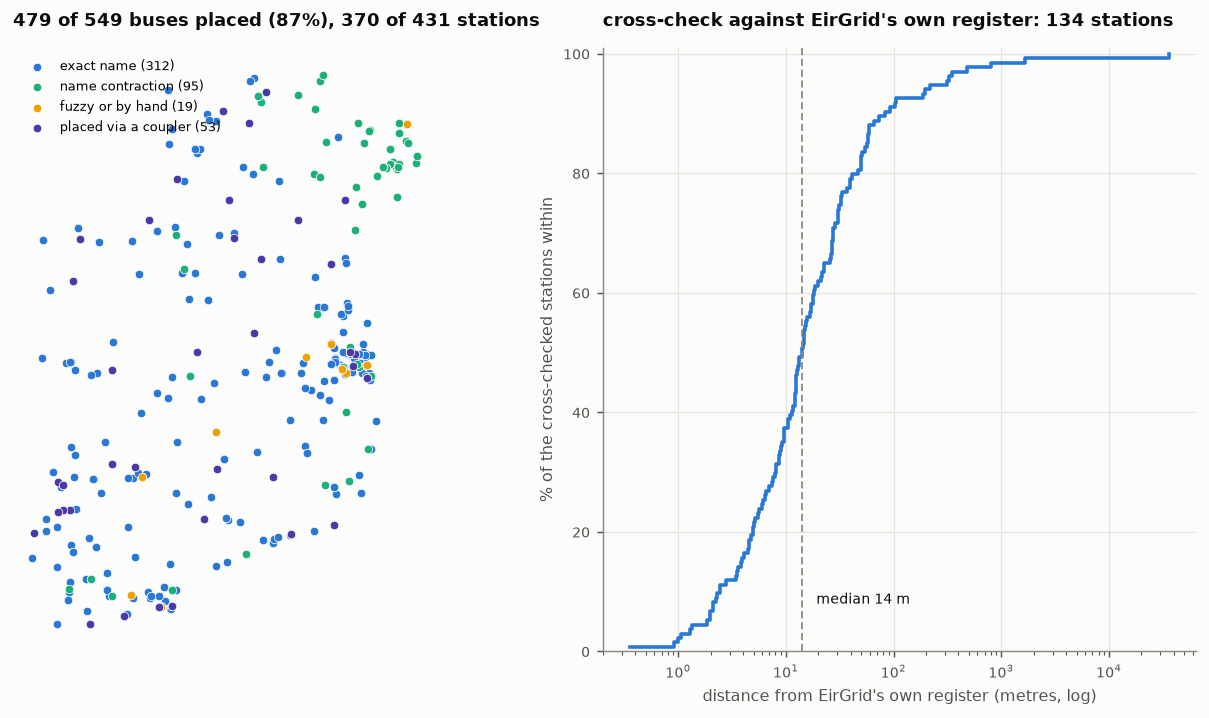
\includegraphics[width=\textwidth]{g_geocoding.png}
\caption{Left: where the WP2024 transmission buses landed, coloured by how each
was matched. Right: the cross-check against the station layer of EirGrid's own
\href{https://services-eu1.arcgis.com/1VGs4Se8lewgdzfE/arcgis/rest/services/TDP_2024_Web_Map_PUBLIC/FeatureServer}{Transmission Development Plan service}. 134 of
the matched stations appear in both, at a median separation of
\textbf{14~metres}, which is the difference between one corner of a substation
and another. The 95th percentile is 252~metres.}
\label{fig:geocode}
\end{figure}

\begin{table}[H]\centering\small
\begin{tabular}{lrl}
\toprule
\textbf{method} & \textbf{buses} & \textbf{what it means} \\
\midrule
\code{exact}      & 309 & normalised names equal, voltage tag agrees \\
\code{coupled}    &  53 & joined to a placed bus by a coupler or its own transformer \\
\code{ni-code}    &  60 & Northern Ireland contraction resolved by subsequence \\
\code{truncated}  &  19 & the twelve-character name is a prefix of exactly one candidate \\
\code{fuzzy}      &  13 & token-sort score $\geq 92$ with $\geq 6$ points over the runner-up \\
\code{prefix}     &  10 & six characters or more, matching exactly one candidate \\
\code{alias}      &   6 & resolved by hand, with the reasoning recorded \\
\code{ni-site}    &   6 & the same Northern Ireland site at its other voltage class \\
\code{exact-name} &   3 & names equal, candidate carries no voltage tag \\
\midrule
\textbf{unplaced} & \textbf{70} & every one named, with its rejected candidate \\
\bottomrule
\end{tabular}
\caption{479 of WP2024's 549 buses placed, which is 87\%. Counts re-derived for
this draft from \file{data/pypsa/geocoding/}. Voltage is corroboration rather
than a key: OpenStreetMap's voltage tag is present on 1{,}270 of the island's
1{,}705 named power objects, so agreement raises confidence, absence does not
lower it, and a contradiction rejects the match.}
\end{table}

\subsection{Two rules that do most of the work}

\textbf{The Northern Ireland contraction.} Buses there are named with a four or
five letter contraction and a digit: \code{ANTR1A}, \code{BAFD2-},
\code{MAGF2-}. The letters are a subsequence of the station's name rather than
a prefix, so BAME is Bally\textbf{me}na, BNCH is Bally\textbf{n}a\textbf{ch}inch
and MAGF is \textbf{Mag}hera\textbf{f}elt. No amount of fuzzy string matching
reaches those, so they are matched by subsequence and scored on how tightly the
letters sit. The trailing digit is a voltage class, 1 for 110~kV and 2 for
275~kV, which holds for every pair the cases contain.

\textbf{Coupling.} A capacitor, reactor, SVC or phase-shifter bus carries a
name of its own, such as \code{MOB\_CAP} or \code{ENNK\_PST}, which no name
match will ever reach because it is not the name of a place. Two things put two
buses inside the same fence: a zero-impedance branch, and a transformer between
two buses both at 110~kV or above, which is the station's own transformer
standing in its yard. Together those place 48 stations that string matching
would have missed.

\subsection{The three hard cases}

\textbf{Cathaleen's Fall} appears in the study files as \code{CATH\_FALL} and
\code{CATH FALL}, because the name does not fit in twelve characters.
OpenStreetMap spells it Cathleen's Fall, without the second `a'. Neither
spelling reaches the other by truncation or by fuzzy matching, so it is in the
alias table with that reasoning written beside it.

\textbf{Clogher} is four separate 110~kV buses in the file and one substation in
OpenStreetMap. The four are busbar sections of one site, which is exactly what
the zero-impedance coupler between two of them says, so they are grouped before
matching and share one coordinate.

\textbf{Clady} is absent from the study files at any voltage, and that is not a
naming problem. OpenStreetMap has a Clady 38~kV substation and a Clady
hydroelectric station in Gweedore, both tagged at 38~kV. EirGrid's own
110~kV-and-above register does not contain it either. A 38~kV station sits
below the transmission model's floor, and Clady's four megawatts do not earn a
bus of their own.

\subsection{The 70 unplaced buses}

Every one is listed with its method, its best rejected candidate and the score.
Fifty-five scored nothing above the threshold, and most are genuinely not in
OpenStreetMap: the island has 367 substations tagged at 110~kV or above against
431 stations in the case, so a residue is expected. Four are ambiguous, where
two candidates cannot be separated: \code{DRUM1} sits equally tightly inside
Drumnakelly and Drumlins Park Wind Farm. Three are rejected because the only
name match is at the wrong voltage class. One is deliberate: SCOTLAND is the GB
end of Moyle, a boundary bus and not a place in Ireland, so it is left without a
coordinate instead of being put at Auchencrosh.

The 2033 cases place 78\% against 87\%. The difference is what the forecast
statement exists for: stations that do not exist yet are not in OpenStreetMap.

\subsection{The one disagreement worth reporting}

Of the 134 cross-checked stations, one is more than 5~km out. TANDRAGEE sits
36.3~km away, and EirGrid's register is the one that is wrong: it puts the
station at the Republic's end of the Louth to Tandragee 275~kV interconnector,
in Co.\ Louth, while the substation is in Co.\ Armagh where OpenStreetMap has
it.

\textbf{A caveat on the validator.} The same feature service is known to be
incomplete on its line layers, as Section~\ref{sec:sources} sets out. The
station layer shows no such gap and the cross-check is station to station, but
a validator with a documented hole in it should be named as one.

\where{geocode.py}{normalise(), \_subsequence\_span(), ALIASES, match(), crosscheck()}

\subsection{The stated line lengths are real, and here is the check}
\label{sec:lengths}

An earlier draft of this report listed the line lengths as placeholders.
Checking it instead of repeating it, and re-deriving the figures for this
draft directly from the raw files:

\begin{itemize}
\item \textbf{83\% of transmission branches carry a non-zero length}, 561 of
      679 in WP2024, with a median of 11.7~km and a longest of 208.5~km.
\item Of the 118 that do not, \textbf{111 are couplers and stubs} with
      $|X| \leq 0.01$, where a zero length is the correct value. Seven are real
      circuits missing a length, and six of those seven are in Northern
      Ireland.
\end{itemize}

\begin{figure}[H]\centering
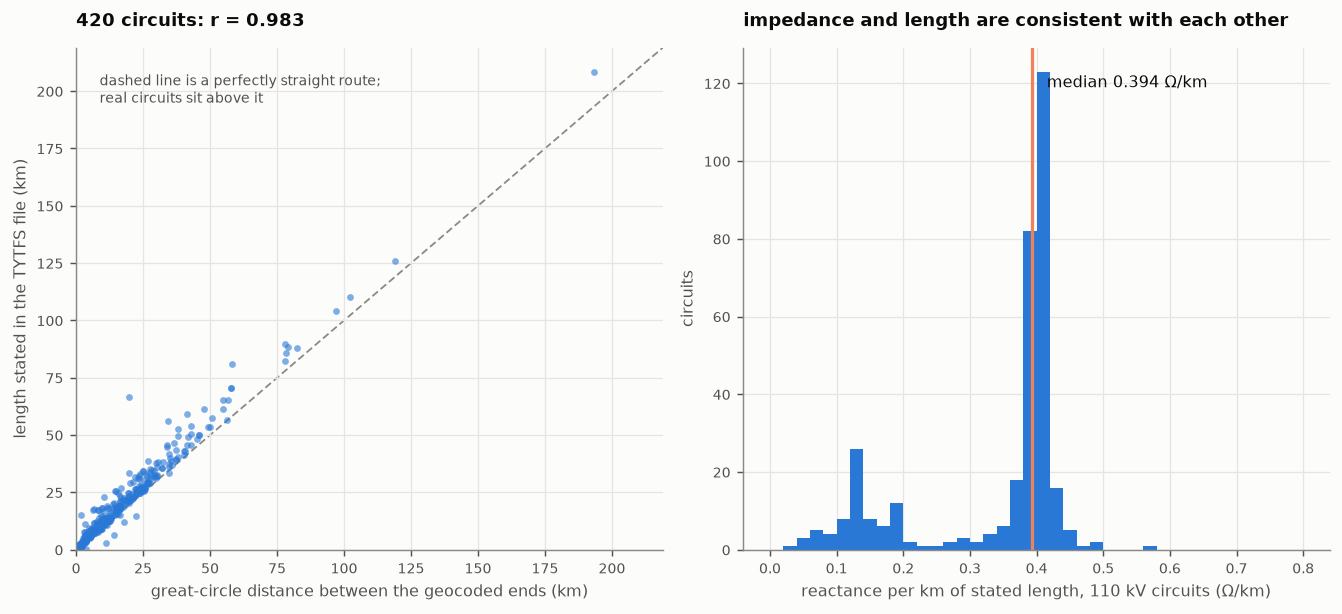
\includegraphics[width=\textwidth]{j_lengths.png}
\caption{Left: for the 420 circuits with a stated length and both ends
independently geocoded, the stated length against the great-circle distance
between the ends. $r = 0.983$, median ratio 1.17, which is what a real route
does against a straight line. Two datasets that share no source agreeing this
closely checks the geocoding as much as it checks the lengths. Right: reactance
per km of stated length at 110~kV.}
\label{fig:lengths}
\end{figure}

The right-hand panel is bimodal, and the split is physical. The 347 circuits
above 0.25~$\Omega$/km have a median of 0.394~$\Omega$/km and a median shunt
susceptance of 0.00035~pu/km. The 117 below have a median of 0.13~$\Omega$/km
and 0.011~pu/km, which is thirty times the charging. High capacitance with low
reactance per km is the signature of underground cable, and the names in that
cluster are Ringsend to Whitebank, Galway to Salthill, Marina to Trabeg: urban
and coastal, where cable is what gets laid.

Two things follow. The lengths are usable, with the seven gaps named. And the
participant kit's fallback of 0.4~$\Omega$/km for a new circuit, which an
earlier draft called a rule of thumb, is within 2\% of the median of this
dataset's own overhead-line population.

% ===================================================================
\clearpage
\section{Part V. The North-West region}
\label{sec:northwest}

EirGrid and SONI run a Wind Dispatch Tool in their control centres, which
applies megawatt limits to individual wind and solar farms or to groups of them
associated with a particular network constraint. The group definitions are
\href{https://cms.eirgrid.ie/sites/default/files/publications/Wind-Dispatch-Tool-Constraint-Group-Overview_0.pdf}{published}. The region studied here is Donegal, Sligo
and north Mayo: heavily wind-dominated, behind a narrow export path, and
identified in the brief as constraint groups 1 to 3.

\textbf{What the published groups are, and why the numbering matters.} The
February 2024 overview lists the North West groups as Letterkenny A1 busbar
flows, Letterkenny A2 busbar flows, Carrick-on-Shannon to Arva, two
outage-driven groups covering Sliabh Bawn to Lanesboro and Binbane to
Cathaleen's Fall, and Corderry to Srananagh, which was retired after that
circuit was uprated. The \href{https://www.sem-o.com/sites/semo/files/documents/wind-dispatch-tool-constraint-groups.pdf}{2020 version} numbered them differently: group 1 was
Letterkenny to Clogher and group 2 Corderry to Srananagh.

Two consequences. The station set studied here is clearly the right region:
Letterkenny, Clogher, Binbane, Cathaleen's Fall, Corderry and Srananagh all
appear in EirGrid's own group definitions. But the numbering is not stable
across versions, so the phrase ``groups 1 to 3'' does not by itself pin down a
fixed set of stations, and nothing here should be read as reproducing a
particular numbered group.

Neither overview document could be retrieved from this environment, since the
hosts are refused by its egress policy, so those group names come from a search
index rather than from the documents. They should be checked against the PDFs
before being quoted onward.

\begin{figure}[H]\centering
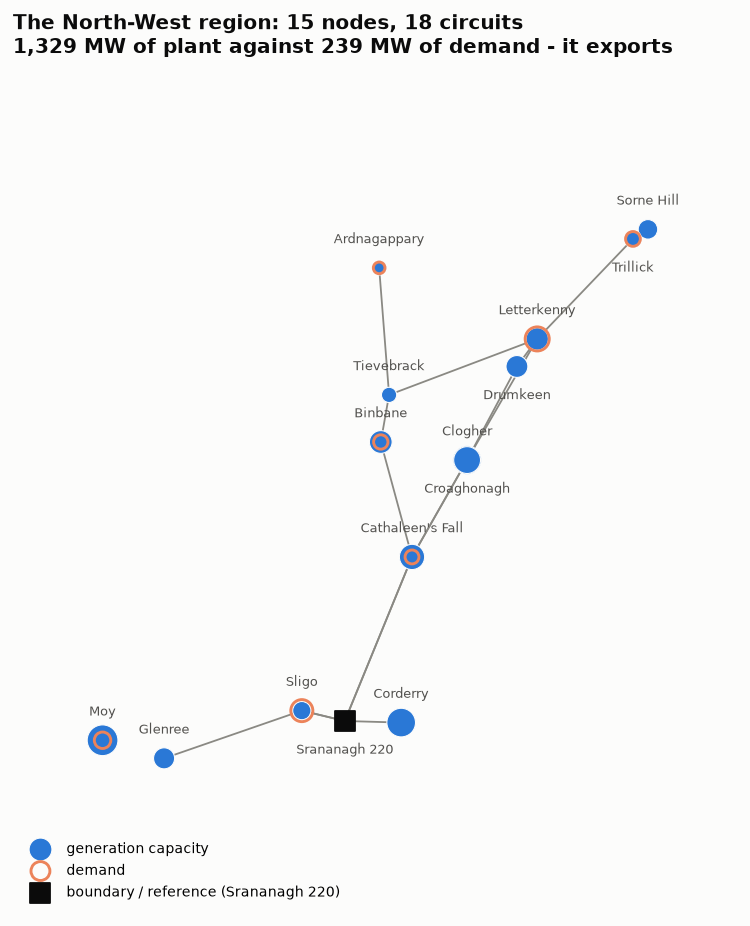
\includegraphics[width=0.82\textwidth]{i_northwest.png}
\caption{The region as the kit ships it. Dot area is plant capacity, the ring
is demand, the square is Srananagh 220~kV, which is both the boundary and the
reference. 1{,}329~MW of plant against 239~MW of demand, so it exports, and the
question is whether the wires can carry it.}
\label{fig:northwest}
\end{figure}

\subsection{Two views, because the two datasets draw a station differently}

The hand-built dataset folds a generator's connection point into the substation
it hangs off. The study files give several of them 110~kV buses of their own.
Both views are therefore produced, and the mapping between them is one table in
the code:

\begin{lstlisting}
STATIONS = (
    Station("Srananagh 220", (5042,), 220.0, note="the region's export path"),
    Station("Srananagh 110", (5041,), 110.0, parent="Srananagh 220"),
    Station("Cathaleen's Fall", (1701, 17010, 17061), 110.0),
    Station("Cliff", (1761,), 110.0, parent="Cathaleen's Fall"),
    ...
)
\end{lstlisting}

The native view is 24 stations, matching the hand-built 24-node block one for
one with a single substitution: the study files have no Clady, and they split
Srananagh into a 110~kV and a 220~kV busbar that the spreadsheet holds as one
node. The aggregated view folds nine of those into their parents and gives the
15 nodes the spreadsheet has.

The region is listed by name instead of being derived, for two reasons. A
constraint group is a published grouping, and not a property of the network
that anyone could compute. And the
region is not the radial island behind Srananagh that a purely topological
definition would find: removing the Srananagh transformer leaves every bus in
the region still connected, through Corderry and Arigna towards Flagford, and
through Letterkenny and Corraclassy into Northern Ireland.

\where{northwest.py}{STATIONS, station\_table(), bus\_map(), extract()}

\subsection{The circuit count}

The brief said 16 circuits among the 15 stations. Reproduced independently:
\textbf{16 routes, carried by 19 circuits}. Both numbers are right and they
answer different questions. A route is a pair of stations and a circuit is a
wire, and three of these routes are double circuits whose two wires land on
different busbars at one or both ends, which is exactly why they collapse to
one edge in a node-and-edge list. The native 24-station view has 25 routes and
29 circuits.

\subsection{What folding to 15 nodes costs}

Same impedances, same injections, a different reference bus: a DC flow has to
put the same megawatts on every circuit as the full network does. That makes
the fold a check with a number attached.

\begin{table}[H]\centering\small
\begin{tabular}{lr}
\toprule
\textbf{what is folded} & \textbf{worst disagreement against the full network} \\
\midrule
nothing (24-station native view)         & \textbf{0.0099 MW} \\
all nine folds (15-station view)         & 21.59 MW \\
all but Srananagh 110                    & \textbf{1.74 MW} \\
all but Srananagh 110, Lenalea, Cunghill & 0.15 MW \\
\bottomrule
\end{tabular}
\caption{Almost all of the error is one fold. Merging Srananagh's two busbars
short-circuits the 250~MVA transformer between them, whose 0.064~pu of
reactance is a large fraction of the region's total, and that redistributes the
two Cathaleen's Fall to Srananagh circuits by 21.6~MW each.}
\end{table}

\textbf{The recommendation is one node.} Split Srananagh back into 110 and
220~kV with the transformer between them, giving 16 nodes instead of 15, and
the flow error falls from 21.6~MW to 1.7. That is a cheap change to a dataset
that is otherwise sound.

\where{northwest.py}{compare\_with\_full(), extract(), verify()}

\subsection{What the reconciliation found in the hand-built data}

\textbf{The wind capacities are right.} Four of the hand-built figures agree
with the study files to within 1\%: Mulreavy at 95 against 95.25, Meentycat 85
against 84.96, Cunghill 35 against 34.80, Lenalea 30 against 30.50. These are
the same numbers rounded.

\textbf{The hydro capacities are all identically 38, and none of them matches.}
Cathaleen's Fall, Cliff and Clady are given 38~MW each. Cathaleen's Fall alone
is two machines of 22.5 and 23~MW in the study files; Cliff is two of 10;
Clady's real rating is about 4.2~MW. All three plants connect at 38~kV, 278
buses in WP2024 carry that voltage, and Cathaleen's Fall has a bus named
\code{HY\_CATH FALL} sitting at exactly 38~kV. A connection voltage entered
into a capacity column is the reading that fits, and it is worth checking
before the 76~MW the spreadsheet puts at Cathaleen's Fall is used for anything.

\textbf{The two blocks of the spreadsheet disagree by exactly 35~MW}, which is
Cunghill. The 24-node block assigns it to Sligo and the 15-node block gives
Sligo no supply at all.

\textbf{The supply set is a correct subset of a larger one.} Every
plant it names is in the study files at the station it says. The study files
carry 1{,}155~MW of connected capacity across those 15 stations against the
spreadsheet's 425~MW, and the gap sits almost entirely at stations the
spreadsheet gives zero supply: Croaghonagh at 139~MW, Moy at 190, Corderry at
145, Binbane at 75. So the region is more export-dominated than the hand-built
data says, at 5.4 to 1 against the hand-built 2.7 to 1.

\textbf{Demand agrees in total and not in distribution.} 160~MW against
213~MW is agreement for a nominal figure against a winter peak. But nine of the
fifteen nodes carry demand in the spreadsheet that the study files put at zero,
because they are transmission stations with no 38~kV load busbar beneath them,
while Letterkenny carries 66~MW in the files against 15 in the spreadsheet.
The pattern is a nominal per-station allocation of 5, 10, 15 or 20~MW against
the case's actual load at the six stations that have any.

\textbf{The 15-node region is a 2024 region.} In both 2033 cases it comes apart,
and not as a modelling artefact: the 2033 network rebuilds the Mayo 110~kV
system. The Glenree to Moy circuit has no record at all, a new station called
Firlough sits between them instead, and Moy gains ties to two other new
stations. Firlough is not in the node set, so Moy falls out of the region and
the extract has two components. \code{northwest.py verify} reports that as a
failure, which is the right answer.

\subsection{Where the constraint actually is}

\code{python northwest.py windy --capacity-factor X} puts the region's capacity
to work at $X$ and re-solves \emph{the whole transmission network}. Not the
extract: an extract with five of its six ties pinned sends every extra megawatt
out through the sixth and gives an answer that is both large and meaningless.

\begin{table}[H]\centering\footnotesize
\setlength{\tabcolsep}{4pt}
\begin{tabular}{lrlrr}
\toprule
\textbf{capacity factor} & \textbf{net export} & \textbf{worst tie} &
\textbf{Srananagh} & \textbf{worst internal} \\
\midrule
10\%  & $-97$ MW (importing) & Letterkenny/Strabane 0.36$\times$ & $-85$ MW & 0.40$\times$ \\
20\%  & 18 MW                & Letterkenny/Strabane 0.71$\times$ & $-62$ MW & 0.48$\times$ \\
\rowcolor{surface}
\textbf{30\%} & \textbf{134 MW} & \textbf{Letterkenny/Strabane 1.05$\times$} & $-39$ MW & 0.56$\times$ \\
60\%  & 480 MW               & Letterkenny/Strabane 2.09$\times$ & $+31$ MW & 0.80$\times$ \\
100\% & 942 MW               & Letterkenny/Strabane 3.48$\times$ & $+123$ MW & \textbf{1.11$\times$} \\
\bottomrule
\end{tabular}
\caption{The binding constraint is the Letterkenny to Strabane 110~kV tie into
Northern Ireland, circuit \code{3581-89516-1}, and it binds at about 29\% of
connected capacity. Srananagh does not reverse into export until about 45\%.
\textbf{The rating is scenario-dependent}: RATE1 on this circuit is 93~MVA in
WP2024, the case this sweep runs on, and 80, 105 and 123~MVA in SV2024, SV2033
and WP2033. All four were re-read from the files for this draft. Quoting one
number for it across scenarios is wrong.}
\label{tab:windy}
\end{table}

So Srananagh 220 is the right place to slack the extraction and the wrong place
to look for the constraint. Two caveats are real and load-bearing: nothing
outside the region is re-dispatched, and the system reference is Turlough Hill,
far away. A study that cares should redo this with the Northern Ireland network
dispatched rather than held fixed.

\subsection{Both north-western cross-border ties sit behind a phase shifter}
\label{sec:pst}

This came out of chasing a numerical discrepancy in the participant kit
(Section~\ref{sec:kit}) and is worth stating on its own. Reading the
transformer records directly, and re-reading them for this draft:

\begin{table}[H]\centering\small
\begin{tabular}{lllrr}
\toprule
\textbf{from} & \textbf{to} & \textbf{rating} & \textbf{shift, winter} &
\textbf{shift, summer} \\
\midrule
89510 STRABANE (NI)  & 89515 STRA\_PST & 125 MVA & $17^\circ$ & $12^\circ$ \\
79010 ENNISKIL (NI)  & 79015 ENNK\_PST & 125 MVA & $3^\circ$  & $3^\circ$ \\
\bottomrule
\end{tabular}
\caption{The only two phase-shifting transformers with both ends at
transmission voltage, present in all four cases. \code{PST} is the file's own
naming. The Strabane angle differs between the winter and summer cases, which
an earlier draft of this report missed by quoting 17$^\circ$ for all four.}
\end{table}

The circuit this report keeps returning to, \code{3581-89516-1}, runs from
Letterkenny to bus 89516, which sits behind 89515 and therefore behind the
phase shifter. The other north-western cross-border tie, Corraclassy to
Enniskillen, has the same arrangement. So the binding element sits directly
behind the device a system operator installs precisely to control flow on a
tie.

\textbf{This model holds both taps fixed.} That is a sharper statement of the
limitation than saying SONI would redispatch around it: there is a specific,
identified control device on the constrained path whose action is not modelled
here.

\where{psse.py}{read\_raw() $\rightarrow$ case.transformer, field ANG1}

\subsection{None of the four published cases runs the fleet}

Worth stating before any of the above is read as a description of the system as
operated. Between 3\% and 21\% of the region's machines are dispatched in any
of the four cases, because these are peak and valley security studies and a
security study does not credit wind. Two of the four cases export, by 23 and
35~MW, against more than a gigawatt of connected capacity. The export the Wind
Dispatch Tool exists to manage does not appear in any of them, which is why the
capacity-factor sweep above exists.

% ===================================================================
\clearpage
\section{Part VI. Turning four snapshots into hours}
\label{sec:hours}

Each case is one hour with a solved dispatch. Anything that asks when the
network is constrained needs a year, and the year has to have weather in it.

\subsection{The pipeline that could not run}

\file{profiles.py} is a complete pipeline against \href{https://open-meteo.com/en/docs/historical-weather-api}{Open-Meteo's historical weather API},
which serves ECMWF's \href{https://doi.org/10.1002/qj.3803}{ERA5 reanalysis} on a 0.25\textdegree{} grid and the
higher-resolution \href{https://doi.org/10.5194/essd-13-4349-2021}{ERA5-Land} on a 0.1\textdegree{} grid, without a key
and under CC BY 4.0.

Reanalysis is the right source for one specific reason. Calm anticyclones and
storm fronts are hundreds of kilometres across and cross Ireland in hours, so
every wind farm in Donegal reaches rated output within the same few hours and
falls to zero within the same few hours. That joint behaviour is what loads a
constrained tie, and a reanalysis has it because it is a reconstruction of what
the atmosphere actually did.

The module does batched requests, caches on disk by grid cell and year so
nothing is fetched twice, computes an hourly shear exponent from the two ERA5
wind levels instead of assuming one, smooths a stated turbine power curve into
a farm curve by \href{https://doi.org/10.1016/j.energy.2016.08.068}{Gaussian convolution}, runs a panel model using the
\href{https://doi.org/10.1016/0038-092X(82)90302-4}{Erbs diffuse-fraction correlation}, allocates
the island demand across buses in proportion to each bus's own load, and
validates the modelled fleet against EirGrid's published all-island wind
series.

\textbf{It has never run}, for the reason given in Section~\ref{sec:blocked}.
Both hosts are refused at the CONNECT.

\textbf{So there are no reanalysis profiles in this repository and no
validation result.} What exists instead is the pipeline, tested, with the fetch
as the only untested step, and every path that cannot get real data raises
instead of falling back on something invented. That behaviour is itself
tested:

\begin{lstlisting}
test_loading_a_cell_that_was_never_fetched_raises
test_a_partial_year_is_not_cached_as_a_complete_one
test_a_response_missing_a_variable_is_refused
test_an_unreadable_eirgrid_file_raises_rather_than_guessing
\end{lstlisting}

The brief was explicit that the validation is the only thing standing between a
real profile and a plausible-looking fabrication. Shipping a generated year
under the ERA5 label, however carefully footnoted, would be that fabrication.

\textbf{Two ways to finish it.} Allowlist the two hosts and re-run: total
traffic is about six HTTP requests per case-year, because sites are
deduplicated to the weather grid before anything is asked for. Or hand-download
a dashboard export into \file{data/raw/eirgrid/} and the Open-Meteo JSON into
\file{data/raw/weather/}, and everything after the fetch runs unchanged.

\textbf{One thing that needs solving either way.} 82 of WP2033's generator
records, carrying 7.8~GW, have no coordinate, and almost all of that is
offshore: Dublin Array, Arklow, the three Codling sites, Kish and Bray, Skerd
Rocks, Oriel. The onshore substation is the wrong coordinate for them, because
the weather at Codling Bank is not the weather at its landfall, and ERA5-Land
does not cover sea in any case. Those sites need real coordinates and the
coarser ERA5 grid, which the module already supports.

\where{profiles.py}{fetch(), load\_cell(), farm\_curve(), solar\_capacity\_factor(), validate\_wind(), Unavailable}

\subsection{The generator that stands in for it}

\file{synthetic.py} produces a deterministic year from the case file alone. It
exists for two reasons: as insurance against exactly the blocker above, and so
that a study can build counterfactuals no historical year contains, such as a
worse wind year or a higher-penetration scenario.

\textbf{The single detail that decides whether it is worth anything is spatial
correlation.} Independent per-bus noise passes almost every test anybody would
write: the profiles land in $[0,1]$, the load factor comes out at 30\%, each
bus looks plausible on its own. And it is useless, because 400 independent
sites average out. The central limit theorem flattens the fleet into a nearly
constant series, and a network that is never asked to carry a surge is never
constrained.

So the wind field is built as a Gaussian random field with an exponential
correlation decay in distance, driven through an Ornstein-Uhlenbeck process in
time with a 36-hour synoptic timescale, mapped onto a Weibull wind speed by a
Gaussian copula, and put through the same power curve the ERA5 path uses:

\[
\rho(d) = \exp\!\left(-\frac{d}{L}\right), \qquad L = 400~\mathrm{km}
\]

\begin{figure}[H]\centering
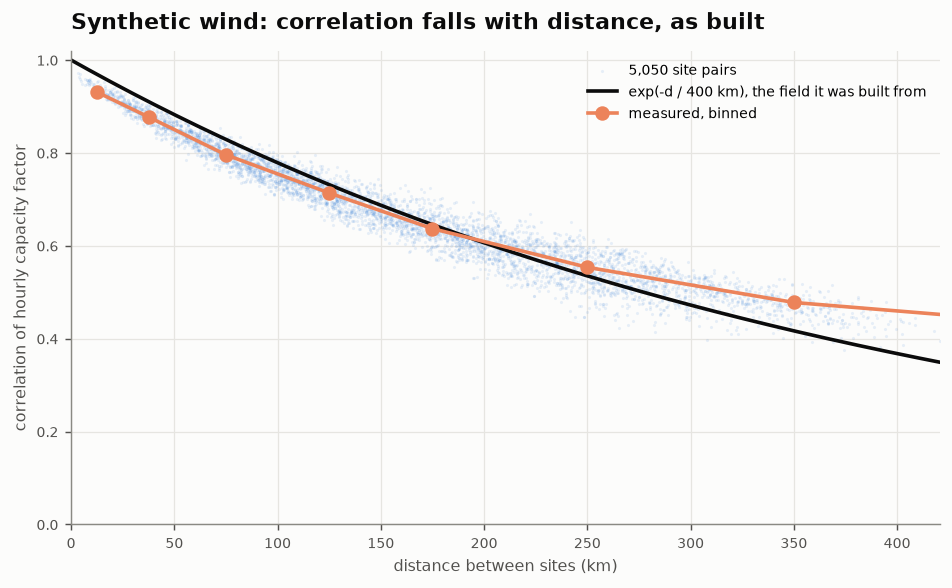
\includegraphics[width=0.85\textwidth]{h_correlation.png}
\caption{The check that matters, measured off the output rather than assumed.
Every pair of wind sites, correlation of hourly capacity factor against
distance. The black curve is the field it was built from and the orange line is
what came out. They agree. Had this come out flat and near zero, every
dispatch-down number in this report would be worthless.}
\label{fig:correlation}
\end{figure}

The other half of the check is that the aggregate has to move. It does: fleet
mean 0.313, standard deviation 0.248, 1{,}053 hours below 5\% of capacity,
486 hours above 80\%, and a longest continuous calm of 112 hours. Independent
noise would give a standard deviation of a couple of points and would never
approach either rail. Two tests assert both halves.

\subsection{Anchored on the four published states}

The generated year is not free-floating. WP2024 and WP2033 are winter-peak
conditions and SV2024 and SV2033 are summer valleys, so each case is placed at
an hour of the year that reproduces its state, and the field tapers back to
unconstrained over 18 hours either side. Demand is rescaled so that the year's
maximum and minimum are that vintage's own two totals, which keeps 2033's
demand out of 2024's year.

\begin{lstlisting}
ANCHOR_POINTS = {"WP": (1, 17, 18), "SV": (7, 9, 5)}   # month, day, hour
ANCHOR_WINDOW_H = 18
SEED = 42
\end{lstlisting}

\textbf{One anchor is deliberately refused.} WP2033 dispatches 373~MW of solar
at a winter-peak evening, a capacity factor of 0.10. At 18:00 on 17 January the
sun is well below the horizon at every Irish latitude, so that value is
unreachable and forcing it would put daylight into the profile at night. The
generator declines it and records why in its anchor report. This is not a fault
in the study files: a case is a set of conditions the network must withstand,
with each carrier's output chosen for the study rather than for a clock.

The same reasoning cuts the other way and should be said plainly. The wind
anchor is applied, so 17 January evening in the generated year is calm because
the case says so. That is a security assumption being written into one hour of
the weather, which is why the window is confined to 18 hours either side.
A year in which every cold evening was calm would be a worse lie than the one
this module replaces, and Irish winter peaks frequently coincide with high
wind.

\subsection{What is real in the generated year, and what is not}

\begin{table}[H]\centering\small
\begin{tabularx}{\textwidth}{lX}
\toprule
\textbf{real} & The network. Which generators exist, what they are, where they
connect and what they are rated at. Which buses carry load and what share of
the island's demand each one carries. Site coordinates. The four anchor states.
The power curve and the panel model, shared with the ERA5 path. \\
\addlinespace
\textbf{generated} & Every hour of weather. The shape of demand through the
day. The hydro and thermal availability shapes. Where in the year the anchors
sit. \\
\addlinespace
\textbf{solved rather than chosen} & The Weibull scale, found by bisection so
that the fleet load factor comes out at the target, which gives 8.40~m/s for
the default settings. The demand scaling, so that the year's extremes are the
case's own. \\
\bottomrule
\end{tabularx}
\caption{The network, the fleet and where the demand sits are real. When
anything happens is invented. A dispatch-down total computed from this is a
statement about a plausible year rather than about any year that occurred.}
\end{table}

\subsection{Does the 2033 case actually bind?}

The whole exercise turns on it. If the profiles do not produce hours where the
network cannot take what the wind offers, the central problem never appears.

\begin{table}[H]\centering\small
\begin{tabular}{lrr}
\toprule
& \textbf{WP2024} & \textbf{WP2033} \\
\midrule
hours studied (windiest) & 60 & 60 \\
energy offered   & 1.4 GWh & 342.8 GWh \\
energy dispatched down & \textbf{0.0 GWh} & \textbf{20.4 GWh} \\
dispatch-down    & 0.0\% & \textbf{5.94\%} \\
hours with dispatch-down & 0 of 60 & \textbf{60 of 60} \\
\bottomrule
\end{tabular}
\caption{It binds, in every hour studied. The 2024 comparison is not a fair
fight and should not be read as one: the WP2024 network is built from
in-service machines and that case runs almost no wind, so it holds a single
wind generator and there are only 1.4~GWh to hold back. What the pair shows is
that the scenario creates the problem and the profile generator does not.}
\end{table}

The single binding circuit, at 100\% of its rating in every hour, is
\code{3581-89516-1}, Letterkenny to Strabane. Section~\ref{sec:northwest}
reached the same circuit from a completely different direction, and
Section~\ref{sec:crossval} is about how much that agreement is worth.

\where{synthetic.py}{correlation\_matrix(), gaussian\_field(), anchors(), taper(), binding()}

% ===================================================================
\clearpage
\section{Part VII. The participant kit}
\label{sec:kit}

\file{participant-kit/} is a standalone directory. It contains no build tooling
and imports nothing from the rest of the repository, so it can be lifted out
whole.

\begin{table}[H]\centering\small
\begin{tabular}{ll}
\toprule
\file{networks/} & 4 scenarios $\times$ 2 scopes, as netCDF and as CSV folders \\
\file{gridkit.py} & load, edit, reset, save, and read results back \\
\file{flowmath.py} & PTDF, susceptibility, shift factors \\
\file{plotstyle.py} & one validated palette for every chart \\
\file{examples/} & six scripts, a to f \\
\file{test\_kit.py} & 20 checks, runnable without pytest \\
\bottomrule
\end{tabular}
\end{table}

\begin{table}[H]\centering\small
\begin{tabular}{lrrrrr}
\toprule
\textbf{scenario} & \textbf{buses} & \textbf{circuits} & \textbf{generators} &
\textbf{week peak demand} & \textbf{capacity} \\
\midrule
WP2024 & 646 & 645 & 295 & 7{,}325 MW & 22{,}650 MW \\
SV2024 & 639 & 640 & 225 & 4{,}948 MW & 14{,}591 MW \\
WP2033 & 754 & 755 & 929 & 8{,}792 MW & 42{,}574 MW \\
SV2033 & 754 & 755 & 264 & 6{,}058 MW & 18{,}283 MW \\
\bottomrule
\end{tabular}
\caption{The all-island networks, read from \file{networks/manifest.csv}. The
generator count includes one load-shedding generator per load bus, which is why
it exceeds the machine count. Capacity excludes those. The four differ in fleet
size because each network is built from its own case's in-service records:
WP2024 carries one wind generator and WP2033 carries 425. WP2033 is the
interesting case, with 42.6~GW of connected plant against an 8.8~GW peak, and
that headroom is where constraint and dispatch-down live.}
\end{table}

Every network carries 168 hourly snapshots, one week centred on the hour that
matches its own case state. Both file formats ship because many participants
would rather edit a spreadsheet than learn an API.

\subsection{The loader}

\begin{lstlisting}
import gridkit

gridkit.quiet()                                  # PyPSA and HiGHS are chatty
n = gridkit.load("WP2033", "all-island")         # or "north-west"

gridkit.add_line(n, "Meentycat", "Srananagh 220", s_nom=200)
gridkit.remove_line(n, "3581-89516-1")
gridkit.set_rating(n, "2781-4951-1", 200.0)
gridkit.add_battery(n, "Letterkenny", p_nom=50, hours=4)

gridkit.solve(n)                                 # n.optimize, log off
print(gridkit.dispatch_down(n).head())
print(gridkit.binding(n).head())

n = gridkit.reset(n)                             # back to the baseline
\end{lstlisting}

\where{participant-kit/gridkit.py}{load(), add\_line(), remove\_line(), set\_rating(), add\_battery(), reset(), dispatch\_down(), binding(), unserved()}

\subsection{Two traps, both already sprung}

Both are in the kit's README, because each cost time to find and neither
announces itself.

\textbf{Freezing the dispatch.} \code{n.optimize()} writes its answer to
\code{generators\_t.p}. \code{n.lpf()} reads \code{generators\_t.p\_set}, which
is a separate table that the kit ships empty. Run the power flow straight after
the optimisation and you get a flow with no generation in it: the reference bus
silently supplies the whole island and one circuit shows at 1600\% of its
rating. \code{gridkit.freeze\_dispatch(n)} copies one into the other.

\textbf{Buses at 0\textdegree{}N 0\textdegree{}E.} PyPSA's netCDF writer turns
a missing coordinate into 0.0 instead of a null, and that point is in the Gulf
of Guinea. Plot the raw bus table and Ireland ends up in the corner of an
Atlantic-to-equator map. \code{gridkit.placed\_buses(n)} drops those and
respects the \code{coordinate\_source} column.

\clearpage
\subsection{(a) DC power flow}

\begin{figure}[H]\centering
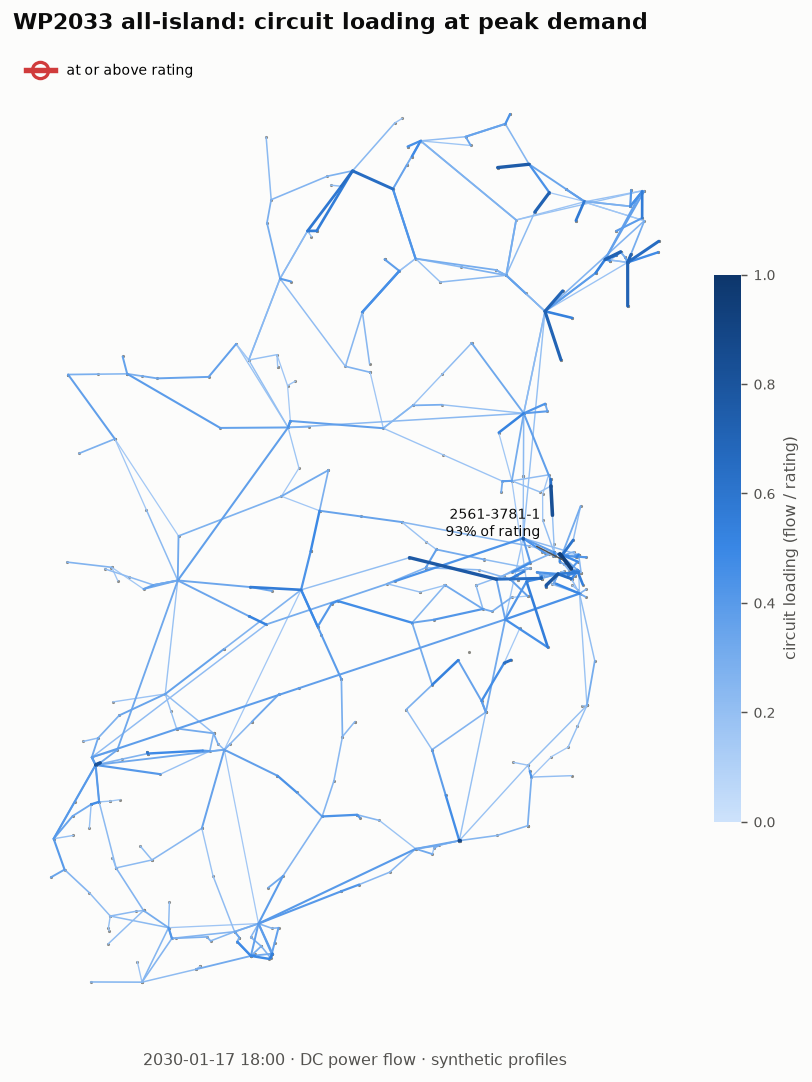
\includegraphics[width=0.72\textwidth]{a_flow_map_WP2033_all-island.png}
\caption{WP2033 at peak demand. Each circuit is coloured by how full it is, and
the one at or over its rating is drawn in red and ringed, because several
circuits join buses a few hundred metres apart and a stroke alone would be
invisible. Nothing here is optimised: a DC power flow takes the dispatch as
given and says where the flow ends up.}
\end{figure}

Six circuits sit at their rating for at least one hour of the week. The worst,
\code{3581-89516-1}, is at 100\% for \textbf{118 of 168 hours}.

\where{participant-kit/examples/a\_dc\_power\_flow.py}{main(), \_draw()}

\clearpage
\subsection{(b) Dispatch, dispatch-down, and how much of it the network caused}

\begin{figure}[H]\centering
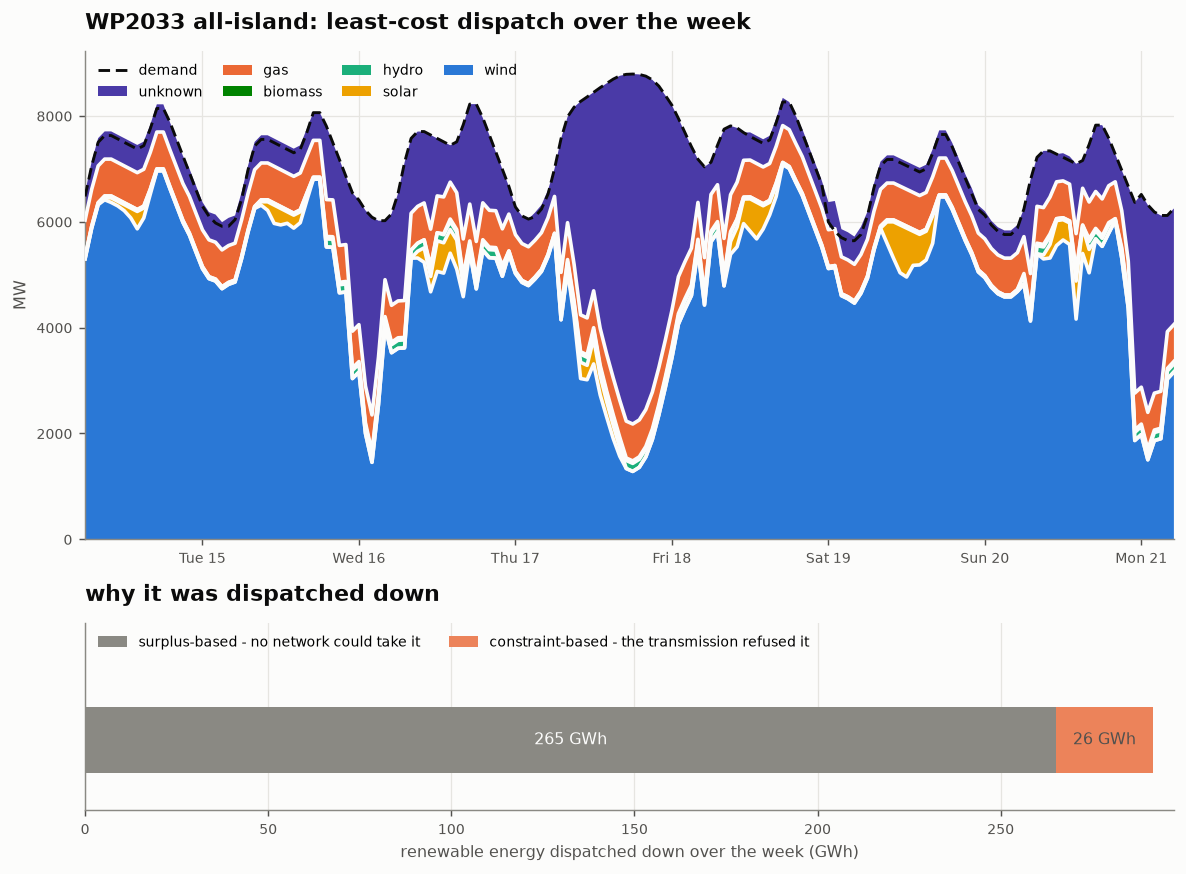
\includegraphics[width=\textwidth]{b_dispatch_WP2033_all-island.png}
\caption{Least-cost dispatch over the week, and the reason for the
dispatch-down.}
\label{fig:dispatch}
\end{figure}

Wind supplies 68\% of the week's energy. 291~GWh of renewable output is
withheld, which reads as a damning verdict on the transmission system until it
is separated. It is worth being precise about what that number is: it is plain
economic dispatch-down, not curtailment in the SEM sense. Curtailment as
EirGrid uses the word is a system-wide, pro-rata reduction of wind and solar
ordered to respect an SNSP or an inertia limit, and there is no SNSP
constraint, no inertia constraint and no unit commitment anywhere in this
model. What the LOPF withholds splits instead by cause, into
\textbf{constraint-based} dispatch-down, stranded behind a specific binding
line rating, and \textbf{surplus-based}, where supply simply exceeds what the
demand can absorb.

\textbf{The separation costs one extra solve.} Lift every branch rating out of
the way and re-optimise. Whatever is still withheld is surplus-based and no
network could have taken it; the difference is constraint-based, and it is
what the transmission cost.

\begin{table}[H]\centering\small
\begin{tabular}{lrl}
\toprule
265.2 GWh & 91\% & surplus-based, from 42.6~GW of plant against an 8.8~GW peak \\
\rowcolor{surface}
\textbf{26.3 GWh} & \textbf{9\%} & \textbf{constraint-based, which is what the network refused} \\
\bottomrule
\end{tabular}
\caption{A large dispatch-down figure does not by itself implicate the network.
In WP2033, building a line recovers none of the 265~GWh. This distinction is
the difference between a headline and a finding.}
\end{table}

\where{participant-kit/examples/b\_lopf\_dispatch.py}{\_congestion\_share(), by\_carrier()}

\clearpage
\subsection{(c) Capacity expansion}

\begin{figure}[H]\centering
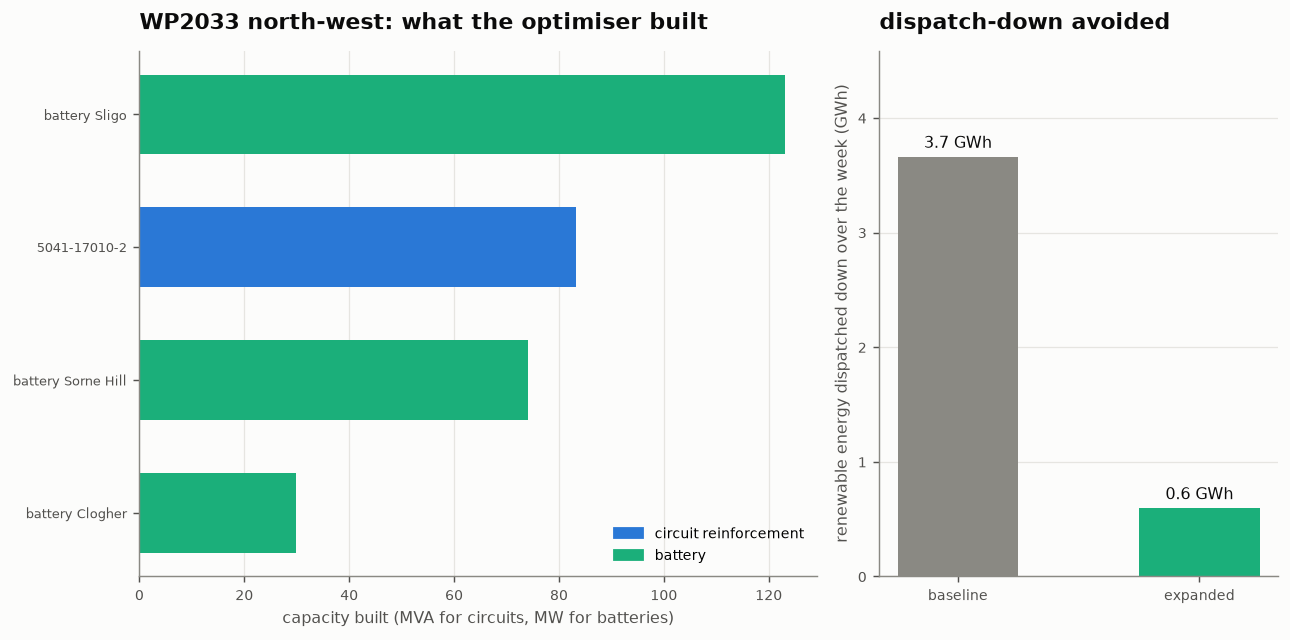
\includegraphics[width=0.92\textwidth]{c_expansion_WP2033_north-west.png}
\caption{The binding circuits are marked extendable, a battery is offered at
every renewable bus, both are given an annualised cost, and the optimiser
trades building against dispatching down.}
\end{figure}

On the North-West region it reinforces one circuit by 83~MVA and builds three
batteries, cutting the week's dispatch-down from 3.7~GWh to 0.6. The costs are
round numbers standing in for a price list. The point is the pattern: mark a
component extendable, give it a capital cost, solve, and read the optimised
rating back.

\where{participant-kit/examples/c\_capacity\_expansion.py}{\_make\_extendable(), \_offer\_batteries()}

\clearpage
\subsection{(d) PTDF from the pseudoinverse}

Everything in \file{flowmath.py} comes out of one object, the weighted graph
Laplacian $L = K B K^{\!\top}$, where $K$ is the bus-branch incidence matrix and
$B$ the diagonal of branch susceptances.

$L$ is singular, because adding a constant to every angle changes no flow, so
it is inverted with the Moore-Penrose pseudoinverse:
\[
\theta = L^{+}(p + KB\varphi), \qquad
F = B\,(K^{\!\top}\theta - \varphi), \qquad
\mathrm{PTDF} = B K^{\!\top} L^{+}
\]

\textbf{Why the pseudoinverse rather than deleting a slack row.} The textbook
fix is to pick a slack, delete its row and column, and invert what is left.
That works, and it writes the arbitrary choice of slack into every number that
comes out. $L^{+}$ returns the solution orthogonal to the nullspace, which is
the one where the balancing megawatt is spread evenly. The choice has not
disappeared; it has become explicit, and \code{shift\_factors()} lets you
change it without rebuilding anything.

\begin{figure}[H]\centering
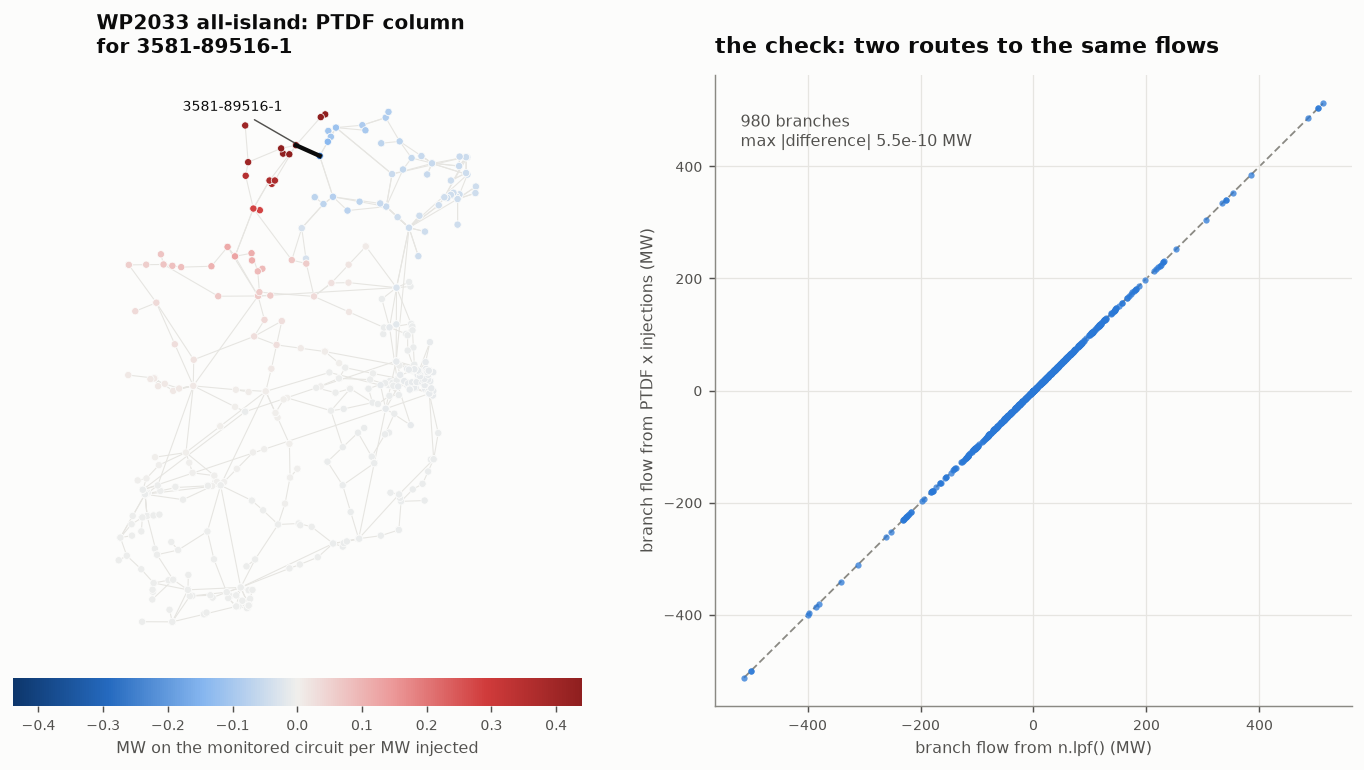
\includegraphics[width=\textwidth]{d_ptdf_WP2033_all-island.png}
\caption{Left: one PTDF column on the map, showing how much of an injection at
each bus the monitored circuit carries. The pale middle of the island is the
part the circuit cannot feel at all. Right: the check. Branch flows rebuilt
from $\mathrm{PTDF}\times p$ against what PyPSA's own linear power flow
produced, over 980 branches. Maximum disagreement $5.5\times10^{-10}$~MW.}
\label{fig:ptdf}
\end{figure}

\textbf{That check earned its keep.} It first came out at \textbf{79~MW}, and
the reason was the network's two phase-shifting transformers, one of them at
17$^\circ$. A phase shifter imposes an angle of its own, so the flow is
$b(\theta_i - \theta_j - \varphi)$ and the bus equation gains a $KB\varphi$
term, which behaves exactly like a pair of equal and opposite injections. The
PTDF itself is unaffected and the flows are not. A PTDF that has not been
checked against a power flow is a matrix of plausible numbers.

\where{participant-kit/flowmath.py}{branches(), laplacian(), pseudoinverse(), ptdf(), angles(), flows()}

\clearpage
\subsection{(e) Edge-to-edge susceptibility, and Braess's paradox}
\label{sec:braess}

Differentiating $F = BK^{\!\top}L^{+}p$ with respect to one branch's
susceptance gives the full edge-to-edge response matrix:
\[
\frac{\partial F_e}{\partial B_{e'}}
= \delta_{ee'}\,a_e \;-\; B_e\left(k_e^{\!\top} L^{+} k_{e'}\right) a_{e'}
\]
where $a_e = F_e/B_e$ is the effective angle difference across branch $e$, that
is the plain angle difference less any phase shift.

The diagonal is the obvious part. The off-diagonal is where \href{https://doi.org/10.1007/BF01918335}{\textbf{Braess's paradox}} lives: a positive entry means that strengthening
$e'$ puts more power on $e$. The effect is established in power networks
specifically, both \href{https://doi.org/10.1088/1367-2630/14/8/083036}{theoretically} and on a real AC laboratory grid with a
\href{https://doi.org/10.1038/s41467-022-32917-6}{topological predictor}. Power in a network is
imposed rather than routed. It divides between parallel paths in inverse
proportion to reactance, and nothing consults the ratings, so building a second
circuit anywhere in a mesh changes every impedance ratio in it.

\begin{figure}[H]\centering
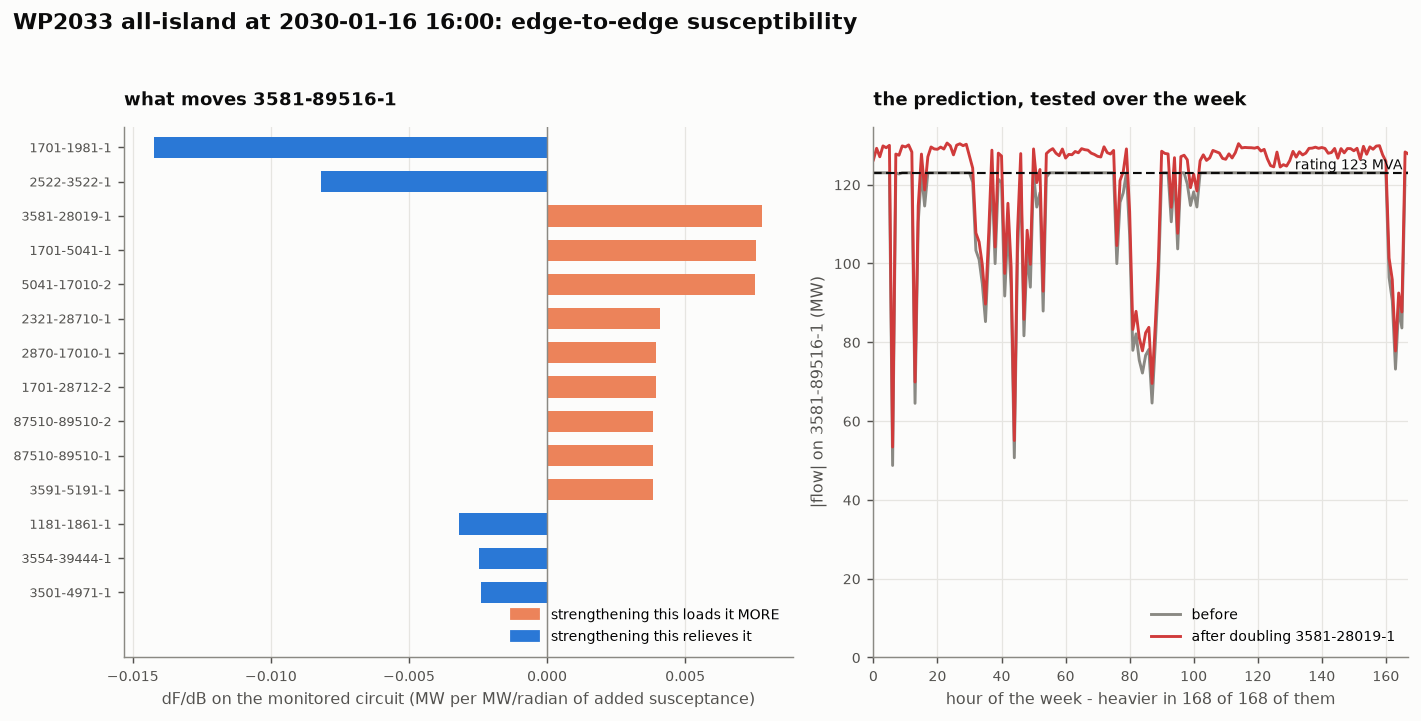
\includegraphics[width=\textwidth]{e_braess_WP2033_all-island.png}
\caption{Left: the branches that move the island's most-loaded circuit, signed.
Of the 979 other branches, strengthening \textbf{516} of them makes it worse.
Right: the derivative is a claim, so the script tests it. It doubles the
susceptance of the strongest candidate, which is what a second circuit on the
same route does, holds the dispatch fixed, and re-solves the flow.}
\label{fig:braess}
\end{figure}

\textbf{The result.} Doubling \code{3581-28019-1} makes \code{3581-89516-1}
carry more power in \textbf{168 of 168 hours}. Flow at the studied hour goes
from 123.0 to 127.3~MW against a 123~MVA rating. A reinforcement a reasonable
planner might propose makes the binding constraint worse.

\where{participant-kit/flowmath.py}{susceptibility(), braess\_candidates()}

\clearpage
\subsection{(f) Shift factors, and what a constraint group looks like}

For one monitored circuit, how much of each generator's output that circuit
carries. Rank the generators by it and the result has the shape of a constraint
group: the machines a dispatch instruction would have to act on.

\textbf{Calling this a reproduction of EirGrid's methodology would overstate
it}, and the heading above comes from the brief's own wording. EirGrid's
\href{https://cms.eirgrid.ie/sites/default/files/publications/Wind-Dispatch-Tool-Constraint-Group-Overview_0.pdf}{published groups} are defined by a monitored flow and are
the product of contingency studies, an AC network and the Northern Ireland
system. What follows is a DC shift-factor ranking on
one intact circuit. It is the right arithmetic and a smaller amount of it.

\begin{figure}[H]\centering
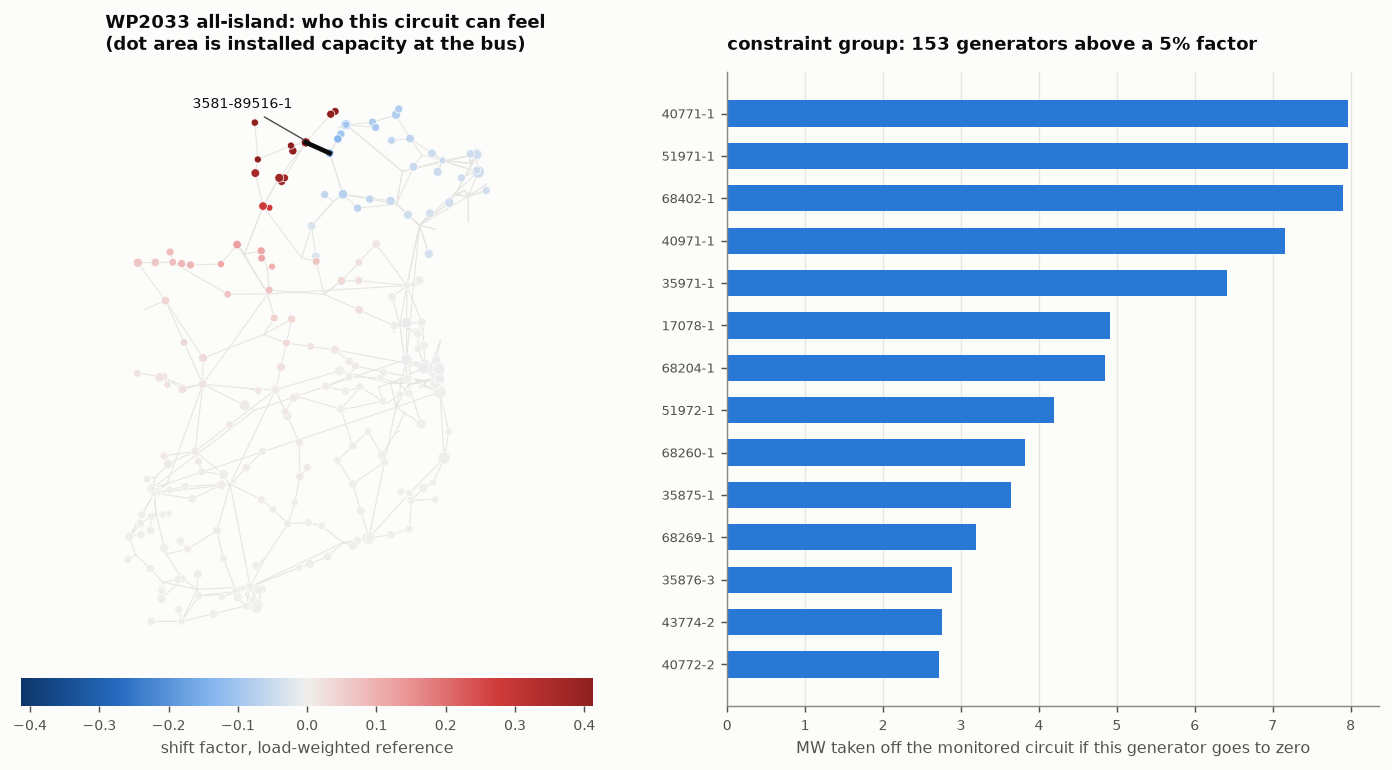
\includegraphics[width=\textwidth]{f_shift_factors_WP2033_all-island.png}
\caption{Left: the shift factor at every bus, with dot area showing installed
capacity. Right: the constraint group, ranked by the megawatts of relief each
member could actually deliver at the studied hour.}
\end{figure}

The thing to be careful about is the reference. A shift factor is megawatts on
the circuit per megawatt at the generator, and a megawatt cannot appear on its
own, so the definition is incomplete until you say where the balancing megawatt
goes. The kit offers three conventions: spread it over every load in proportion
to size, which is what a system operator means; spread it evenly over all
buses, which is the pseudoinverse's own reference; or put all of it at one
named bus, which is the textbook single-slack convention.

\textbf{The values differ and the ranking does not.} Spearman rank correlation
between the three references is \textbf{1.0000}. That invariance is why the
method is robust enough to run a real dispatch tool on, and it is worth knowing
that it is an invariance rather than a coincidence.

\where{participant-kit/flowmath.py}{shift\_factors()}

% ===================================================================
\clearpage
\section{Findings}

\subsection{Two independent methods agree on the binding circuit}
\label{sec:crossval}

This is the result worth the most, because nothing was tuned to produce it.

\begin{table}[H]\centering\small
\begin{tabularx}{\textwidth}{lXX}
\toprule
& \textbf{Section~\ref{sec:northwest}} & \textbf{Sections~\ref{sec:hours} and~\ref{sec:kit}} \\
\midrule
network   & 2024 & 2033 \\
method    & DC power flow, other ties pinned at the case's own values &
            full linear optimisation over a week \\
profiles  & none, a capacity-factor sweep & generated correlated weather \\
scope     & the North-West region & the whole island \\
\midrule
rating of that circuit & 93 MVA in WP2024 & 123 MVA in WP2033 \\
\midrule
\textbf{answer} & \multicolumn{2}{c}{\cellcolor{surface}\textbf{\code{3581-89516-1},
Letterkenny to the Strabane phase-shifter bus}} \\
\bottomrule
\end{tabularx}
\caption{Different network vintage, different method, different data, no shared
code beyond the conversion itself. Same circuit.}
\end{table}

\textbf{How much this is worth, stated carefully.} The two methods share the
conversion, the geocoding and the topology. They are independent in vintage,
dispatch, profiles and scope rather than in everything. The agreement is also
partly structural: the region exports and this is its narrowest export path, so
a thermal-limit method was always likely to land here. What the agreement rules
out is that the finding is an artefact of the generated weather or of the 2033
build-out. It does not establish that this is the constraint a control room
would act on.

Independent support from outside this work: EirGrid's two live North West
\href{https://cms.eirgrid.ie/sites/default/files/publications/Wind-Dispatch-Tool-Constraint-Group-Overview_0.pdf}{constraint groups} in February 2024 both monitor Letterkenny busbar
flows, and the circuit found here is one of the circuits on
that busbar. That corroborates the area rather than the specific circuit, and
Section~\ref{sec:northwest} explains why it cannot be more than that.

\subsection{Most dispatch-down in the 2033 case is not the network's fault}

Of 291~GWh dispatched down in WP2033, 265 is surplus-based and 26 is
constraint-based. The instinct on seeing a large figure is to propose
reinforcement. In this scenario, 91\% of it would be money spent on energy
that has nowhere to go regardless.

\subsection{Reinforcement can make a constraint worse, and here is a case}

Of the 979 branches that could be strengthened, 516 would increase the flow on
the island's most-loaded circuit. The strongest candidate, verified on a
re-solved power flow, makes it worse in every hour of the week. This is a
reason to compute the susceptibility matrix before proposing a circuit.

\subsection{Below 38 kV, OpenStreetMap cannot supply a distribution network}

Section~\ref{sec:osm}. 2\% of distribution transformers, 6{,}707 medium-voltage
components against a true figure near 571, and no snapping tolerance that
recovers the missing spans. Above 38~kV the same data is good and is free.

\subsection{Four things about the hand-built North-West dataset}

Restated because they are actionable: the hydro capacities are the 38~kV
connection voltage rather than capacities; the 24-node and 15-node blocks
differ by exactly Cunghill's 35~MW; splitting Srananagh back into two nodes
takes the model's flow error from 21.6~MW to 1.7; and the node set describes
the 2024 network, coming apart in both 2033 cases where a new station replaces
the Glenree to Moy circuit.

% ===================================================================
\clearpage
\section{Bugs found, and what each one cost}

Each of these produced a network that ran. That is the reason to write them
down.

\begin{enumerate}[leftmargin=1.5em]

\item \textbf{Every optimisation infeasible.} PyPSA 1.x turns a non-null
\code{p\_set} into a hard equality that pins the dispatch. The networks carried
the case's own dispatch, which is the case's answer asserted, and it is
infeasible against a lossless model. Fixed by a function that clears it and
keeps the case's values in a column of their own.

\item \textbf{The full network still infeasible.} The coupler-bounding rule,
applied to sub-110~kV distribution transformers, produced limits that bind on
the case's own flows on 13 transformers, worst at 156\%. Fixed by restricting
the rule to zero-impedance couplers.

\item \textbf{WP2033's angles out by 100$^\circ$.} PyPSA's own slack choice
survived a per-label assignment and one 21~MW hydro machine absorbed 856~MW.
Section~\ref{sec:slack}. Angle correlation 0.90 to 0.99.

\item \textbf{The optimisation exported 1{,}223~MW for profit.} A single
bidirectional generator with a positive marginal cost and a negative lower
bound gets paid to run backwards. Split into an import generator and an export
sink.

\item \textbf{7.8~GW of wind running flat out.} 82 wind and solar generators in
WP2033 had no availability series, because the generated weather is produced at
geocoded sites and their buses never matched OpenStreetMap. PyPSA defaults a
missing series to 1.0, so at a zero bid they ran at full output for all 168
hours: more than the island's peak demand, a fifth of the fleet, must-run
baseload labelled wind. The dispatch-down figure read 64\% instead of 26\%. Each
now borrows the nearest profile of its own carrier. \textbf{The dispatch chart
looked entirely reasonable throughout.}

\item \textbf{The North-West had no wind at all.} The extraction folded every
machine at a station into one generator with a single carrier, which was right
for the reconciliation it was written for. For the kit it meant a region that
is 90\% wind could not be dispatched down. Now split by carrier from the case's own
machine records.

\item \textbf{Flows out by 79~MW.} The two phase-shifting transformers, caught
only because the PTDF was checked against a power flow.

\item \textbf{A circuit at 1600\% of its rating.} A power flow run after an
optimisation without freezing the dispatch. Now a named function, with the
symptom described in its docstring so the next person recognises it.

\item \textbf{Ireland in the corner of a map of the Atlantic.} Three buses at
0\textdegree{}N 0\textdegree{}E.

\item \textbf{Guards that never fired.} Several checks were testing the row
count of an empty-column DataFrame, which is the snapshot count and always
truthy, so the dispatch-freezing helper would silently freeze nothing.

\end{enumerate}

% ===================================================================
\section{Tests}

\begin{lstlisting}[language=shell]
python -m pytest                            # 215 passed
cd participant-kit && python test_kit.py    # 20/20, no pytest needed
\end{lstlisting}

\begin{table}[H]\centering\small
\begin{tabular}{lrl}
\toprule
\textbf{file} & \textbf{tests} & \textbf{what it guards} \\
\midrule
\file{test\_network.py}   & 37 & the OpenStreetMap layer and the graph builder \\
\file{test\_profiles.py}  & 32 & the ERA5 pipeline, and that it refuses to invent \\
\file{test\_synthetic.py} & 31 & correlation, anchoring, determinism \\
\file{test\_psse.py}      & 30 & the raw-file parser, against the files themselves \\
\file{test\_pypsa\_net.py} & 26 & every conversion decision in Section~\ref{sec:conversion} \\
\file{test\_northwest.py} & 21 & the station map, the circuit count, both views \\
\file{participant-kit/test\_kit.py} & 20 & the kit: networks, loader, linear algebra \\
\file{test\_geocode.py}   & 18 & normalisation, contraction codes, accept and reject rules \\
\midrule
& \textbf{215} & \\
\bottomrule
\end{tabular}
\caption{Counts from the last recorded full run. The machine this draft was
written on has neither PyPSA nor pytest installed, so the suite was not re-run
for it.}
\end{table}

\subsection{The two that matter most}

Most tests check that code does what it says. These two check it against
something that does not share code with it.

\code{test\_ptdf\_matches\_a\_power\_flow} rebuilds every branch flow from
$\mathrm{PTDF}\times p$ and compares it against PyPSA's own linear power flow.
Two routes to the same number, agreeing to $10^{-6}$~MW. This is the test that
found the phase shifters.

\code{test\_susceptibility\_matches\_finite\_differences} perturbs one branch's
susceptance by a ten-thousandth and checks the analytic derivative against the
difference it actually makes:

\begin{lstlisting}
numeric = (flows_with(bumped) - reference) / step
predicted = analytic.iloc[:, column].to_numpy()
# The natural scale is MW per MW/radian.  Some columns are exactly zero,
# because a radial stub's susceptance changes no flow anywhere, so the
# column's own magnitude is not a usable denominator on its own.
scale = max(np.abs(predicted).max(), np.abs(reference).max() / base[column])
assert np.abs(numeric - predicted).max() / scale < 1e-4
\end{lstlisting}

If either drifts, nothing built on \file{flowmath.py} means anything.

% ===================================================================
\clearpage
\section{Limitations}

Read this before presenting anything from it.

\textbf{This is a DC approximation of an AC model.} The study files are full AC
load-flow cases with reactive power, voltage magnitudes, tap changers and shunt
compensation. All of that is discarded here: flows are linear in angle
differences, voltages are 1.0 per unit everywhere, losses are zero. That is the
standard approximation for transmission constraint work and it is good to a few
percent on real flows, but it says nothing about voltage, reactive support or
stability, and a conclusion that depends on those has no support here.

\textbf{Ratings are the file's RATE1 column, and the reading of that column is
an inference.} See Section~\ref{sec:rate}. Beyond that, a control room works to
seasonal, weather-dependent and often dynamic limits that are not in these
files, and runs circuits above the continuous rating for defined periods. A
figure of 100\% of rating here means 100\% of a planning number under an
inferred interpretation of which column that is. Ratings also change between
scenarios: the circuit this report follows is rated 80, 93, 105 and 123~MVA
across the four cases.

\textbf{Line lengths are usable, with seven named gaps.} 83\% of transmission
branches carry a length, it correlates at $r = 0.983$ with the great-circle
distance between independently geocoded endpoints, and reactance per km
separates cleanly into overhead line and cable. Seven real circuits in WP2024
carry no length, six of them in Northern Ireland, and a per-km calculation
should skip those instead of treating a zero as a distance.

\textbf{Every time series is generated.} No hour in them ever happened. They
are anchored so that each network's own scenario hour reproduces the case
state, and the spatial correlation is measured off the output, but they are
neither a historical year nor a forecast. Generators
without a geocoded site borrow a neighbour's profile, which makes those pairs
perfectly correlated when they should not be.

\textbf{This model reports dispatch-down, not curtailment.} Renewable output
that is offered and not taken here is plain economic dispatch-down, and it
splits into constraint-based, stranded behind a binding line rating, and
surplus-based, where supply exceeds what the demand can absorb. It is not
curtailment as the Single Electricity Market and EirGrid use the word: that is
a system-wide, pro-rata reduction of wind and solar ordered to respect an SNSP
or an inertia limit, and this model carries no SNSP constraint, no inertia
constraint and no unit commitment. Nothing here reproduces that mechanism, and
no number in this report should be compared against a published curtailment
figure.

\textbf{Costs are placeholders, and renewables bid negative.} Gas 90, biomass
40, hydro 1 and imports 150~EUR/MWh, with wind and solar at $-1$. The
load-shedding generators bid 10{,}000~EUR/MWh, a round number chosen to sit far
above everything else. It carries no relation to the Single Electricity
Market's \href{https://www.semcommittee.com/publications/sem-23-072-calculation-single-value-lost-load-within-single-electricity-market}{Value of Lost Load}, which was EUR 12{,}533/MWh for 2022.
The negative bid is deliberate, because it is how a support scheme makes a wind
farm willing to pay to stay on, and it makes dispatch-down a last resort
rather than a free choice. It also makes the objective negative, so only differences
between two objectives mean anything.

\textbf{About a fifth of generation carries the carrier \code{unknown}.}
Carriers are inferred from bus-name prefixes and a keyword list, because the
files do not label plant by technology. Any result turning on the split between
\code{gas} and \code{unknown} is unsupported.

\textbf{The DC links are simplified.} Fixed efficiency, no ramp limits, no
minimum stable export, no market coupling. Interconnector flow here is what the
cost assumptions make of it rather than what the day-ahead market would do.

\textbf{One circuit binds, the far side is an infinite sink, and there is an
unmodelled control device on the constrained path.} The model prices export to
Northern Ireland at nothing beyond the tie's thermal limit. In reality SONI,
the \href{https://www.soni.ltd.uk/about-us/what-we-do}{Northern Ireland transmission system operator}, would redispatch
around it, and the tie terminates behind a phase-shifting transformer whose tap
this model holds fixed (Section~\ref{sec:pst}). What the result establishes is
that the profiles produce binding constraints and where, not that any
particular dispatch-down percentage is right.

\textbf{The OpenStreetMap layers are a claim about mapping.} Blank areas below
38~kV mean unmapped rather than unserved, and the county-to-county variation in
mapped density measures mapper effort. Section~\ref{sec:osm} is the detail.

\textbf{The study file data is EirGrid's, provided for reference purposes
only.} It describes a planning forecast. It does not describe the operational
system, and it is published without warranty as to accuracy or fitness for any
particular purpose. Nothing here is an EirGrid product or an EirGrid position.

% ===================================================================
\section{What this draft changed, and what could not be checked here}
\label{sec:corrections}

This draft rewrote the previous one to cover the whole repository instead of
the model build alone, and to put the provenance of every input in one place
near the front. Section~\ref{sec:sources} is the part that did not exist
before.

Numbers were re-derived where the environment allowed it. The machine this was
written on has no scientific Python stack, so anything requiring PyPSA or
pandas was carried across from the recorded runs and is attributed as such.
What was re-derived directly from the source files, with a small standalone
parser, is listed here so a reader knows which is which:

\begin{itemize}
\item The system base of 100~MVA and 50~Hz, from each case's header line.
\item The branch record counts and the equality of RATE1 and RATE2 across all
      4{,}841 records, and the three values RATE3/RATE1 takes.
\item The transmission branch counts, the length statistics, and the split
      between zero-length couplers and real circuits missing a length.
\item The 18 unrated transmission branches in WP2024.
\item The rating of the Letterkenny to Strabane circuit in all four cases.
\item The transformer record assembly, checked by arithmetic, and the two
      phase-shifting transformers with both ends at transmission voltage.
\item The geocoding method counts, placement rates and cross-check distances,
      from the committed CSVs.
\item The OpenStreetMap candidate counts and the county sweep totals, from the
      committed CSVs.
\end{itemize}

\textbf{Two corrections.} The phase-shift angle at Strabane is 17$^\circ$ in
the two winter cases and 12$^\circ$ in the two summer cases; the previous draft
quoted 17$^\circ$ for all four. And the participant kit's own README still
carries the sentence ``Line lengths are placeholders'', which
Section~\ref{sec:lengths} showed to be wrong. That file should be corrected to
match.

\subsection{How sources are cited, and what could not be verified from here}

This report carries no bibliography. Every source is a link on the phrase that
names it, so a reader can go straight to the thing being claimed rather than to
an entry that asserts the thing exists. That is deliberate: a bibliography can
carry an entry nobody ever resolved, and a link either opens or it does not.
Every link in this document was checked to resolve before it was written in.

What checking a link does not establish is that its contents were read here.
Stated plainly, because a source the author could not open is weaker than one
they could.

\begin{itemize}
\item \textbf{Every EirGrid, SONI and SEM-O host is refused by this
      environment's egress policy}, as are the reanalysis and dashboard hosts.
      So the study file landing page, both Wind Dispatch Tool overviews and the
      Value of Lost Load paper are linked as located publications; their
      contents reached this document through a search index rather than through
      the documents themselves. The group names in Section~\ref{sec:northwest}
      are the claim most exposed to that.
\item \textbf{The PSS/E format itself.} Siemens' manual is not public. The bus
      type codes are corroborated by an \href{https://powsybl.readthedocs.io/projects/powsybl-core/en/latest/grid_exchange_formats/psse/}{independent open-source reader};
      the rating semantics are not corroborated by anything, which is why they
      are presented as an inference.
\item \textbf{Nothing in the study files was checked against the physical
      system.} Where this report says a circuit is rated at 93~MVA, it means
      the file says so.
\item \textbf{ESB Networks' asset counts} are quoted from its published
      description of its own network and were not independently checked.
\end{itemize}

% ===================================================================
\clearpage
\section{Where everything is}

\begin{table}[H]\centering\small
\begin{tabular}{lll}
\toprule
\textbf{file} & \textbf{lines} & \textbf{what it does} \\
\midrule
\multicolumn{3}{l}{\color{inksoft}\textit{the coverage study}} \\
\file{network.py}     &  766 & the OpenStreetMap layer and the graph builder \\
\file{eirgrid.py}     &  379 & EirGrid's asset register and county boundaries \\
\file{analysis.py}    &  541 & the five measurements behind \file{FINDINGS.md} \\
\file{plots.py}       &  430 & the national map and one per study area \\
\file{extract\_web\_data.py} & 166 & lines and point assets for the web map \\
\file{extract\_web\_base.py} & 128 & coastline and county outlines \\
\file{build\_web\_map.py}    & 377 & one self-contained HTML file \\
\midrule
\multicolumn{3}{l}{\color{inksoft}\textit{the model build}} \\
\file{psse.py}        &  675 & reads PSS/E v35 raw files, Section~\ref{sec:psse} \\
\file{pypsa\_net.py}  & 1352 & the conversion, Section~\ref{sec:conversion} \\
\file{geocode.py}     & 1085 & OpenStreetMap matching, Section~\ref{sec:geocode} \\
\file{northwest.py}   &  958 & the region, Section~\ref{sec:northwest} \\
\file{profiles.py}    &  948 & the ERA5 pipeline, never run \\
\file{synthetic.py}   &  964 & the generated year, Section~\ref{sec:hours} \\
\file{build\_kit.py}  &  459 & assembles the participant kit \\
\midrule
\multicolumn{3}{l}{\color{inksoft}\textit{the kit, which imports none of the above}} \\
\file{participant-kit/gridkit.py}   & 345 & the loader \\
\file{participant-kit/flowmath.py}  & 340 & PTDF, susceptibility, shift factors \\
\file{participant-kit/plotstyle.py} &  99 & the palette \\
\file{participant-kit/test\_kit.py} & 300 & the checks \\
\file{participant-kit/examples/}    &     & six scripts, a to f \\
\midrule
\multicolumn{3}{l}{\color{inksoft}\textit{documents}} \\
\file{FINDINGS.md}              & 432 & the coverage verdict, in full \\
\file{docs/PHASE1\_PARSER.md}   & 292 & the file format and its validation \\
\file{docs/PHASE2\_PYPSA.md}    & 605 & every conversion decision, with its evidence \\
\file{docs/PHASE3\_NORTHWEST.md} & 474 & the reconciliation, table by table \\
\file{docs/PHASE4\_PROFILES.md} & 338 & the ERA5 pipeline and the blocker \\
\file{docs/SYNTHETIC\_DATA.md}  & 333 & what is real and what is fabricated \\
\file{docs/report/}             &     & this document, its figures and its sources \\
\bottomrule
\end{tabular}
\caption{This report is the summary. The phase documents are the working notes,
and where a number here has a longer story, that is where it is.}
\end{table}

\subsection{Outputs worth knowing about}

\begin{table}[H]\centering\small
\begin{tabularx}{\textwidth}{lX}
\toprule
\file{data/national\_network.png} & both layers over the Republic \\
\file{data/ireland\_distribution\_map.html} & the same distribution layer,
interactive, opens from disk \\
\file{data/eirgrid\_transmission.gpkg} & EirGrid's 110~kV-and-above lines and
stations \\
\file{data/analysis.json}, \file{national.json}, \file{county\_sweep.csv} &
the coverage measurements \\
\file{data/osm\_substations.csv} & the 1{,}705 named OpenStreetMap objects the
matching runs against \\
\file{data/pypsa/<case>\_<scope>/} & each case as a PyPSA CSV folder, with a
report table per decision \\
\file{data/pypsa/geocoding/<case>.csv} & where each bus is, how it was matched,
and why the rest were not \\
\file{data/pypsa/northwest\_<case>\_<view>/} & the region in both views, with
circuits, boundary flows and the comparison against the full network \\
\file{participant-kit/networks/} & the eight shipped networks \\
\bottomrule
\end{tabularx}
\end{table}

\vspace{4mm}
\noindent\textbf{Reproducing every figure in this document.}

\begin{lstlisting}[language=shell]
python plots.py national                       # the map in Part I
python docs/report_figures.py                  # the four build-half figures
cd participant-kit
for e in examples/*.py; do python "$e"; done   # the six kit figures
cd ../docs/report && ./build.sh                # pdflatex x3
\end{lstlisting}

\end{document}
